\ifx\wholebook\relax \else
% ------------------------ 

\documentclass{article}
%------------------- Other types of document example ------------------------
%
%\documentclass[twocolumn]{IEEEtran-new}
%\documentclass[12pt,twoside,draft]{IEEEtran}
%\documentstyle[9pt,twocolumn,technote,twoside]{IEEEtran}
%
%-----------------------------------------------------------------------------
%%
% loading packages
%
\newif\ifpdf
\ifx\pdfoutput\undefined % We're not running pdftex
  \pdffalse
\else
  \pdftrue
\fi
%
%
\ifpdf
  \RequirePackage[pdftex,%
            CJKbookmarks,%
       bookmarksnumbered,%
              colorlinks,%
          linkcolor=blue,%
              hyperindex,%
        plainpages=false,%
       pdfstartview=FitH]{hyperref}
\else
  \RequirePackage[dvipdfm,%
             CJKbookmarks,%
        bookmarksnumbered,%
               colorlinks,%
           linkcolor=blue,%
               hyperindex,%
         plainpages=false,%
        pdfstartview=FitH]{hyperref}
  \AtBeginDvi{\special{pdf:tounicode GBK-EUC-UCS2}} % GBK -> Unicode
\fi
\usepackage{hyperref}

% other packages
%-----------------------------------------------------------------------------
\usepackage{graphicx, color}
\usepackage{CJK}
%
% for programming 
%
\usepackage{verbatim}
\usepackage{listings}


\lstdefinelanguage{Smalltalk}{
  morekeywords={self,super,true,false,nil,thisContext}, % This is overkill
  morestring=[d]',
  morecomment=[s]{"}{"},
  alsoletter={\#:},
  escapechar={!},
  literate=
    {BANG}{!}1
    {UNDERSCORE}{\_}1
    {\\st}{Smalltalk}9 % convenience -- in case \st occurs in code
    % {'}{{\textquotesingle}}1 % replaced by upquote=true in \lstset
    {_}{{$\leftarrow$}}1
    {>>>}{{\sep}}1
    {^}{{$\uparrow$}}1
    {~}{{$\sim$}}1
    {-}{{\sf -\hspace{-0.13em}-}}1  % the goal is to make - the same width as +
    %{+}{\raisebox{0.08ex}{+}}1		% and to raise + off the baseline to match -
    {-->}{{\quad$\longrightarrow$\quad}}3
	, % Don't forget the comma at the end!
  tabsize=2
}[keywords,comments,strings]

\lstloadlanguages{C++, Lisp, Smalltalk}

% ======================================================================

\def\BibTeX{{\rm B\kern-.05em{\sc i\kern-.025em b}\kern-.08em
    T\kern-.1667em\lower.7ex\hbox{E}\kern-.125emX}}

\newtheorem{theorem}{Theorem}

%
% mathematics
%
\newcommand{\be}{\begin{equation}}
\newcommand{\ee}{\end{equation}}
\newcommand{\bmat}[1]{\left( \begin{array}{#1} }
\newcommand{\emat}{\end{array} \right) }
\newcommand{\VEC}[1]{\mbox{\boldmath $#1$}}

% numbered equation array
\newcommand{\bea}{\begin{eqnarray}}
\newcommand{\eea}{\end{eqnarray}}

% equation array not numbered
\newcommand{\bean}{\begin{eqnarray*}}
\newcommand{\eean}{\end{eqnarray*}}

\RequirePackage{CJK,CJKnumb,CJKulem,CJKpunct}
% we use CJK as default environment
\AtBeginDocument{\begin{CJK*}{GBK}{song}\CJKtilde\CJKindent\CJKcaption{GB}}
\AtEndDocument{\clearpage\end{CJK*}}

%
% loading packages
%
\newif\ifpdf
\ifx\pdfoutput\undefined % We're not running pdftex
  \pdffalse
\else
  \pdftrue
\fi
%
%
\ifpdf
  \RequirePackage[pdftex,%
       bookmarksnumbered,%
              colorlinks,%
          linkcolor=blue,%
              hyperindex,%
        plainpages=false,%
       pdfstartview=FitH]{hyperref}
\else
  \RequirePackage[dvipdfm,%
        bookmarksnumbered,%
               colorlinks,%
           linkcolor=blue,%
               hyperindex,%
         plainpages=false,%
        pdfstartview=FitH]{hyperref}
\fi
\usepackage{hyperref}

% other packages
%-----------------------------------------------------------------------------
\usepackage{graphicx, color}
%
% for programming 
%
\usepackage{verbatim}
\usepackage{listings}
\usepackage{algorithmic} %for pseudocode
\usepackage{algorithm}


\lstdefinelanguage{Smalltalk}{
  morekeywords={self,super,true,false,nil,thisContext}, % This is overkill
  morestring=[d]',
  morecomment=[s]{"}{"},
  alsoletter={\#:},
  escapechar={!},
  literate=
    {BANG}{!}1
    {UNDERSCORE}{\_}1
    {\\st}{Smalltalk}9 % convenience -- in case \st occurs in code
    % {'}{{\textquotesingle}}1 % replaced by upquote=true in \lstset
    {_}{{$\leftarrow$}}1
    {>>>}{{\sep}}1
    {^}{{$\uparrow$}}1
    {~}{{$\sim$}}1
    {-}{{\sf -\hspace{-0.13em}-}}1  % the goal is to make - the same width as +
    %{+}{\raisebox{0.08ex}{+}}1		% and to raise + off the baseline to match -
    {-->}{{\quad$\longrightarrow$\quad}}3
	, % Don't forget the comma at the end!
  tabsize=2
}[keywords,comments,strings]

\lstloadlanguages{C++, Lisp, Haskell, Python, Smalltalk}

% ======================================================================

\def\BibTeX{{\rm B\kern-.05em{\sc i\kern-.025em b}\kern-.08em
    T\kern-.1667em\lower.7ex\hbox{E}\kern-.125emX}}

\newtheorem{theorem}{Theorem}

%
% mathematics
%
\newcommand{\be}{\begin{equation}}
\newcommand{\ee}{\end{equation}}
\newcommand{\bmat}[1]{\left( \begin{array}{#1} }
\newcommand{\emat}{\end{array} \right) }
\newcommand{\VEC}[1]{\mbox{\boldmath $#1$}}

% numbered equation array
\newcommand{\bea}{\begin{eqnarray}}
\newcommand{\eea}{\end{eqnarray}}

% equation array not numbered
\newcommand{\bean}{\begin{eqnarray*}}
\newcommand{\eean}{\end{eqnarray*}}




\setcounter{page}{1}

\begin{document}

\fi
%--------------------------

% ================================================================
%                 COVER PAGE
% ================================================================

\title{Trie and Patricia with Functional and imperative implementation}

\author{Liu~Xinyu
\thanks{{\bfseries Liu Xinyu } \newline
  Email: liuxinyu95@gmail.com \newline}
%  Tel:   +86-1305-196-8666 \newline}
  }

\markboth{Trie and Patricia}{Imperative and Functional}

\maketitle

\ifx\wholebook\relax
\chapter{Trie and Patricia with Functional and imperative implementation}

\section{abstract}
\else
\begin{abstract}
\fi
Trie and Patricia are important data structures in
information retreiving and manipulating. None of these data structures
are new. They were invented in 1960s. This post collects some
existing knowledge about them. Some functional and imperative
implementation are given in order to show the basic idea of these data structures.
There are multiple programming languages used, including, C++, Haskell, python and scheme/lisp.
C++ and python are mostly used to show the imperative implementation, while Haskell and Scheme are
used for functional purpose.

There may be mistakes in the post, please feel free to point out.

This post is generated by \LaTeXe, and provided with GNU FDL(GNU Free Documentation License).
Please refer to http://www.gnu.org/copyleft/fdl.html for detail.

\ifx\wholebook\relax\else
\end{abstract}
\fi

\vspace{3cm}
{\bfseries Keywords:} Trie, Patricia, Radix tree

%{\bfseries Corresponding Author:} Liu Xinyu

\maketitle

% ================================================================
%                 Introduction
% ================================================================
\section{Introduction}
\label{introduction}

There isn't a seperate chapter about Trie or Patricia
in CLRS book. While these data structure are very basic, especially in
information retrieving. Some of them are also widely used in
compiler design\cite{okasaki-int-map}, and bio-information area, such as
DNA pattern matching \cite{wiki-suffix-tree}.

In CLRS book index, Trie is redirected to Radix tree, while Radix tree
is described in Problem 12-1 \cite{CLRS}.

\begin{figure}[htbp]
       \begin{center}
	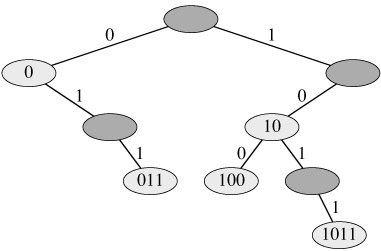
\includegraphics[scale=0.5]{img/radix-tree.eps}
        \caption{an Radix tree example in CLRS} \label{fig:radix-tree}
       \end{center}
\end{figure}

Figure \ref{fig:radix-tree} shows a radix tree contains the bit
strings 1011, 10, 011, 100 and 0. When searching for a key $k=b_0b_1...b_n$, we
take the first bit $b_0$ (MSB from left), check if it is 0 or 1, if it
is 0, we turn left, and turn right for 1. Then we take the 2nd bit and
repeat this search until we either meet a leaf or finish all n bits.

Note that radix tree needn't store key in node at all. The
infomation are represented by edges in fact. The node with key string
in the above figure are only for illustration.

It is very natural to come to the idea `is it possible to represent
keys in integers instead of string, because integer can be denoted in
binary format?'. Such approach can save spaces and it is fast if we
can use bitwise manipulation.

I'll first show the integer based Trie data structure and implementation in
section \ref{int-trie}. Then we can point out the drawbacks and go to
the improved data structure of integer based Patricia in
section \ref{int-patricia}.
After that, I'll show alphabetic Trie and Patricia and list some
typicall use of them in textual manipulation engineering problems.

This article provides example implementation of Trie and Patricia 
in C, C++, Haskell, Python, and Scheme/Lisp languages. Some functional
implementation can be referenced from current Haskell packages \ref{hackage-int-map} 
\ref{hackage-bytestring-map}.

All source code can be downloaded in appendix \ref{appendix}, please 
refer to appendix for detailed information about build and run.

% ================================================================
%                 Int Trie
% ================================================================
\section{Integer Trie}
\label{int-trie}

Let's give a definition of the data structure in figure \ref{fig:radix-tree}.
To be more accurate, it should be called as \emph{binary trie}. a binary
trie is a binary tree in which the placement of each key is controlled by
its bits, each 0 means ``go left at the next node'' and each 1 means ``go
right at the next node''\cite{okasaki-int-map}.

Because integers can be represented in binary format in computer, it is 
possible to store integer keys rather than 0,1 strings. When we insert an
integer as a new key to the trie, we take first bit, if it is 0, we recursively
insert the other bits to the left sub tree; if it is 1, we insert into right
sub tree.

However, there is a problem if we treat the key as integer. Consider a binary
trie shows in figure \ref{fig:big-endian-trie}. If the keys are represented in 
string based on '0' and '1', all the three keys are different. While if they are
turned into integers, they are identical. So if we want to insert a data with integer
key 3, where should we put it into the trie?

\begin{figure}[htbp]
       \begin{center}
	\includegraphics[scale=0.5]{img/big-endian-trie.ps}
        \caption{a big-endian trie} \label{fig:big-endian-trie}
       \end{center}
\end{figure}

One approach is to treat all prefix zero as effective bits.
Suppose an integer is represented in 32-bits, If we want to insert key 1 to a trie, 
it will end up with a 32-levels tree. 
There are 31 node has only 1 left sub tree and the last node has
a right sub tree. It is very inefficent in terms of space.

Chris Okasaki shows a method to solve this problem in \cite{okasaki-int-map}. Instead of 
normal big-endian integer, we can use little-endian integer as key. By using little-endian,
decimal integer 1 is represent as binary 1, if we insert it to an empty binary trie, we
get a trie with a root and a right leaf. There is only 1 level. For integer 3, it is 11 in 
birnary, we needn't add any prefix 0, the position in the trie is unique.

%=========================================================================
%       Definition of integer trie
%=========================================================================
\subsection{Definition of Integer Trie}
Trie is invented by Edward Fredkin. It comes from ``retrieval'', pronouces 
as /'tri:/ by the inventor, while it is pronouced /'trai/ ``try'' 
by other authors \cite{wiki-trie}.
The definition of little-endian binary trie is simple, we can reuse the structure
of binary tree, with its left sub tree to store 0 part and right tree to store 1 part.
The augment data can be stored as value.

\subsubsection*{Definition of little-endian integer Trie in C++}
We can utilize C++ template to abstract the value stored in Trie. The type
of key is integer. Each node contains a value, a left child and a right child.

\lstset{language=C++}
\begin{lstlisting}
template<class T>
struct IntTrie{
  IntTrie():value(), left(0), right(0){}
  ~IntTrie(){
    delete left;
    delete right;
  }
  T value;
  IntTrie* left;
  IntTrie* right;
};
\end{lstlisting}

In order to simplify the release, recursive destruction is added.

\subsubsection*{Definition of little-endian integer Trie in Haskell}
In trie, since a node may not contains value, so we use Haskell Maybe data to represent
this situation. A IntTrie node is either an empty node, or a branch node. The branch
node contains a left child a `Maybe' value and a right child. 

\lstset{language=Haskell}
\begin{lstlisting}
data IntTrie a = Empty 
               | Branch (IntTrie a) (Maybe a) (IntTrie a) -- left, value, right

type Key = Int

-- helpers
left :: IntTrie a -> IntTrie a
left (Branch l _ _) = l
left Empty = Empty

right :: IntTrie a -> IntTrie a
right (Branch _ _ r) = r
right Empty = Empty

value :: IntTrie a -> Maybe a
value (Branch _ v _) = v
value Empty = Nothing
\end{lstlisting}

In order to access the children and value some helper functions are given.

\subsubsection*{Definition of little-endian integer Trie in Python}
The definition of integer trie in Python is shown as below. All fileds
are initialized as empty values.

\lstset{language=Python}
\begin{lstlisting}
class IntTrie:
    def __init__(self):
        self.value = None
        self.left = self.right = None
\end{lstlisting}

left child and right child represent sub Trie branches, and value is used to 
store actual data.

\subsubsection*{Definition of little-endian integer Trie in Scheme/Lisp}
In Scheme/Lisp, we provides some helper functions to create and access 
Trie data. The underground data structure is still list.

TODO: Scheme version of help functions.

% ================================================================
%               Insertion of integer trie
% ================================================================
\subsection{Insertion of integer trie}

\subsubsection{Iterative insertion algorithm}
Since the key is little-endian, when we insert a key into trie, we take the
bit from right most (LSB). If it is 0, we go to the left child, and go to right
for 1. if the child is empty, we need create new node, and repeat this until
meet the last bit (MSB) of the integer. Below is the iterative algorithm
of insertion.

%\begin{algorithm}
\begin{algorithmic}
\STATE $INT-TRIE-INSERT(T, x, data)$
\IF{$T = NIL$}
   \STATE $T \leftarrow EmptyNode$ \ENDIF

  \STATE $p=T$
  \WHILE{$x \neq 0$}
    \IF{$EVEN(x) = TRUE$}
      \STATE $p \leftarrow LEFT(p)$
    \ELSE
      \STATE $p \leftarrow RIGHT(p)$
    \ENDIF
    \IF{$p = NIL$}
      \STATE $p \leftarrow EmptyNode$ \ENDIF
    \STATE $x \leftarrow x/2$
  \ENDWHILE
  \STATE $DATA(p) \leftarrow data$
\end{algorithmic}
%\end{algorithm}

\subsubsection*{Insertion of integer Trie in C++}
With C++ language we can speed up the above even/odd test and key update with
bitwise operation.

\lstset{language=C++}
\begin{lstlisting}
template<class T>
IntTrie<T>* insert(IntTrie<T>* t, int key, T value=T()){
  if(!t)
    t = new IntTrie<T>();

  IntTrie<T>* p = t;
  while(key){
    if( (key&0x1) == 0){
      if(!p->left) p->left = new IntTrie<T>();
      p = p->left;
    }
    else{
      if(!p->right) p->right = new IntTrie<T>();
      p = p->right;
    }
    key>>=1;
  }
  p->value = value;
  return t;
}
\end{lstlisting}

In order to verify this program, some helper functions are provided to
simplify the repeat insertions. And we also provide a function to convert
the Trie to readable string.

\begin{lstlisting}
template<class T, class Iterator>
IntTrie<T>* list_to_trie(Iterator first, Iterator last){
  IntTrie<T>* t(0);
  for(;first!=last; ++first)
    t = insert(t, *first);
  return t;
}

template<class T, class Iterator>
IntTrie<T>* map_to_trie(Iterator first, Iterator last){
  IntTrie<T>* t(0);
  for(;first!=last; ++first)
    t = insert(t, first->first, first->second);
  return t;
}

template<class T>
std::string trie_to_str(IntTrie<T>* t, int prefix=0, int depth=0){
  std::stringstream s;
  s<<"("<<prefix;
  if(t->value!=T())
    s<<":"<<t->value;
  if(t->left)
    s<<", "<<trie_to_str(t->left, prefix, depth+1);
  if(t->right)
    s<<", "<<trie_to_str(t->right, (1<<depth)+prefix, depth+1);
  s<<")";
  return s.str();
}
\end{lstlisting}

Function list\_to\_trie just inserts keys, all values are treated as default
value as type T, while map\_to\_trie inserts both keys and values repeatly.
Function trie\_to\_str helps to convert a Trie to literal string in a modified
pre-order traverse.

The verification cases are as the following.

\begin{lstlisting}
const int lst[] = {1, 4, 5};
std::list<int> l(lst, lst+sizeof(lst)/sizeof(int));

IntTrie<int>* ti = list_to_trie<int, std::list<int>::iterator>(l.begin(), l.end());
std::copy(l.begin(), l.end(), 
          std::ostream_iterator<int>(std::cout, ", "));
std::cout<<"==>"<<trie_to_str(ti)<<"\n";
    
IntTrie<char>* tc;
typedef std::list<std::pair<int, char> > Dict;
const int  keys[] = {4, 1, 5, 9};
const char vals[] = "bacd";
Dict m;
for(int i=0; i<sizeof(keys)/sizeof(int); ++i)
  m.push_back(std::make_pair(keys[i], vals[i]));
tc = map_to_trie<char, Dict::iterator>(m.begin(), m.end());
std::copy(keys, keys+sizeof(keys)/sizeof(int),
          std::ostream_iterator<int>(std::cout, ", "));
std::cout<<"==>"<<trie_to_str(tc);
\end{lstlisting}

The above code lines will output results in console like this.
\begin{verbatim}
1, 4, 5, ==>(0, (0, (0, (4))), (1, (1, (5))))
4, 1, 5, 9, ==>(0, (0, (0, (4:b))), (1:a, (1, (1, (9:d)), (5:c))))
\end{verbatim}

\subsubsection*{Insertion of integer trie in Python}
Imperative implementation of insertion in Python can be easily given by translating
the pseudocode of the algorithm.

\lstset{language=Python}
\begin{lstlisting}
def trie_insert(t, key, value = None):
    if t is None:
        t = IntTrie()

    p = t
    while key != 0:
        if key & 1 == 0:
            if p.left is None:
                p.left = IntTrie()
            p = p.left
        else:
            if p.right is None:
                p.right = IntTrie()
            p = p.right
        key = key>>1
    p.value = value
    return t
\end{lstlisting}

In order to test this insertion program, some test helpers are provided:

\begin{lstlisting}
def trie_to_str(t, prefix=0, depth=0):
    to_str = lambda x: "%s" %x
    str="("+to_str(prefix)
    if t.value is not None:
        str += ":"+t.value
    if t.left is not None:
        str += ", "+trie_to_str(t.left, prefix, depth+1)
    if t.right is not None:
        str += ", "+trie_to_str(t.right, (1<<depth)+prefix, depth+1)
    str+=")"
    return str

def list_to_trie(l):
    t = None
    for x in l:
        t = trie_insert(t, x)
    return t

def map_to_trie(m):
    t = None
    for k, v in m.items():
        t = trie_insert(t, k, v)
    return t
\end{lstlisting}

Function trie\_to\_str can print the contents of trie in pre-order,
It doesn't only print the value of the ndoe, but also print the edge information.

Function list\_to\_trie can repeatly insert a list of keys into a trie, since the
default argument of value is None, so all data relative to keys are empty. If the
data isn't empty, function map\_to\_trie can insert a list of key-value pairs into 
the trie.

Then a test classe is given to encapasulate test cases:

\begin{lstlisting}
class IntTrieTest:
    def run(self):
        self.test_insert()

    def test_insert(self):
        t = None
        t = trie_insert(t, 0);
        t = trie_insert(t, 1);
        t = trie_insert(t, 4);
        t = trie_insert(t, 5);
        print trie_to_str(t)
        t1 = list_to_trie([1, 4, 5])
        print trie_to_str(t1)
        t2 = map_to_trie({4:'b', 1:'a', 5:'c', 9:'d'})
        print trie_to_str(t2)

if __name__ == "__main__":
    IntTrieTest().run()
\end{lstlisting}

Running this program will print the following result.

\begin{verbatim}
(0, (0, (0, (4))), (1, (1, (5))))
(0, (0, (0, (4))), (1, (1, (5))))
(0, (0, (0, (4:b))), (1:a, (1, (1, (9:d)), (5:c))))
\end{verbatim}

Please note that by pre-ordre traverse trie, we can get a 'lexical' order
result of the keys. For instance, the last result print the little-endian
format of key 1, 4, 5, 9 as below.

\begin{verbatim}
001
1
1001
101
\end{verbatim}

They are in lexcical order. We'll go back to this feature of trie later in 
alphabetic trie section.

\subsubsection{Recursive insertion algorithm}
Insertion can also be implemented in a recursive manner. If the LSB is 0, it 
means that the key to be inserted is an even number, we recursively insert the
date to left child, we can devide the number by 2 and round to integer to get
rid of the LSB. If the LSB is 1, the key is then an odd number, the recursive
insertion will be happened to right child. This algorithm is described as below.

\begin{algorithmic}
\STATE $INT-TRIE-INSERT'(T, x, data)$
  \IF { x = 0}
    \STATE $VALUE(T) \leftarrow data$
  \ELSE
    \IF {$EVEN(x)$}
      \STATE $LEFT(T) \leftarrow INT-TRIE-INSERT'(LEFT(T), x/2, data)$
    \ELSE
      \STATE $RIGHT(T) \leftarrow INT-TRIE-INSERT'(RIGHT(T), x/2, data)$
    \ENDIF
  \ENDIF
  \RETURN $T$
\end{algorithmic}

\subsubsection*{Insertion of integer Trie in Haskell}
To simply the problem, If user insert a data with key already exists, we simply
overwrite the previous stored data. This approach can be easily replaced with 
other methods, such as storing data as a linked list etc.

Insertion integer key into a trie can be implementated with Haskell as below.

\lstset{language=Haskell}
\begin{lstlisting}
insert :: IntTrie a -> Key -> a -> IntTrie a
insert t 0 x = Branch (left t) (Just x) (right t)
insert t k x = 
  if even k
       then Branch (insert (left t) (k `div` 2) x) (value t) (right t)
       else Branch (left t) (value t) (insert (right t) (k `div` 2) x)
\end{lstlisting}

If the key is zero, we just insert the data to current node, in other
cases, the program go down along the trie according to the last bit
of the key.

To test if this program, some test helper functions are provided.

\begin{lstlisting}
fromList :: [(Key, a)] -> IntTrie a
fromList xs = foldl ins Empty xs where
    ins t (k, v) = insert t k v

-- k = ... a2, a1, a0 ==> k' = ai * m + k, where m=2^i
toString :: (Show a)=>IntTrie a -> String
toString t = toStr t 0 1 where
    toStr Empty k m = "."
    toStr tr k m = "(" ++ (toStr (left tr) k (2*m)) ++
                      " " ++ (show k) ++ (valueStr (value tr)) ++
                      " " ++ (toStr (right tr) (m+k) (2*m)) ++ ")"
    valueStr (Just x) = ":" ++ (show x)
    valueStr _ = ""
\end{lstlisting}

fromList function can create a trie from a list of integer-data pairs.
toString function can turn a trie data structure to readable string
for printing. This is a modified in-order tree traverse, since the number
stored is in little-endian, the program store the $2^m$ to calculate
the keys. The following code shows a test.

\begin{lstlisting}
main = do
  putStrLn (toString (fromList [(1, 'a'), (4, 'b'), (5, 'c'), (9, 'd')]))
\end{lstlisting}

This will output:
\begin{verbatim}
(((. 0 (. 4:'b' .)) 0 .) 0 (((. 1 (. 9:'d' .)) 1 (. 5:'c' .)) 1:'a' .))
\end{verbatim}

Figure \ref{int-trie} shows this result. 
\begin{figure}[htbp]
       \begin{center}
	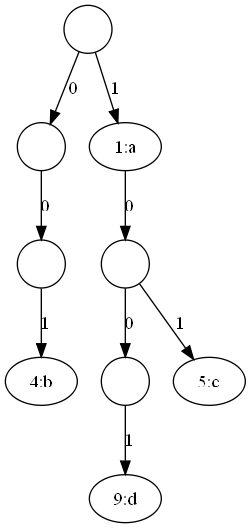
\includegraphics[scale=0.5]{img/int-trie.ps}
        \caption{An little-endian integer binary trie for the map 
          \{$ 1 \rightarrow a, 4 \rightarrow b, 5 \rightarrow c, 9 \rightarrow d$\}.} 
        \label{fig:int-trie}
       \end{center}
\end{figure}


% ================================================================
%               Look up in integer binary trie
% ================================================================
\subsection{Look up in integer binary trie} 

\subsubsection{Iterative looking up algorithm}

To look up a key in a little-endian integer binary trie. We take each
bit of the key from left (LSB), and go left or right according to if
the bit is 0, untill we consumes all bits. this algorithm can be described
as below pseudocode.

\begin{algorithmic}
\STATE $INT-TRIE-LOOKUP(T, x)$
  \WHILE{$x \neq 0$ and $T \neq NIL$}
    \IF{$EVEN(x) = TRUE$}
      \STATE $T \leftarrow LEFT(T)$
    \ELSE
      \STATE $T \leftarrow RIGHT(T)$
    \ENDIF
    \STATE $x \leftarrow x/2$
  \ENDWHILE
  \IF{$T \neq NIL$} \RETURN $DATA(T)$
  \ELSE \RETURN $NIL$ \ENDIF
\end{algorithmic}

\subsubsection*{Look up implemented in C++}
In C++, we can test the LSB by using bitwise operation. The following code
snippet searches a key in an integer Trie. If the target node is found, the
value of that node is returned, else it will return the default value of the
value type\footnote{One good alternative is to raise exception if not found}.
\lstset{language=C++}
\begin{lstlisting}
template<class T>
T lookup(IntTrie<T>* t, int key){
  while(key && t){
    if( (key & 0x1) == 0)
      t = t->left;
    else
      t = t->right;
    key>>=1;
  }
  if(t)
    return t->value;
  else
    return T();
}
\end{lstlisting}

To verify this program, some simple test cases are provided.

\begin{lstlisting}
std::cout<<"\nlook up 4: "<<lookup(tc, 4)
         <<"\nlook up 9: "<<lookup(tc, 9)
         <<"\nlook up 0: "<<lookup(tc, 0);
\end{lstlisting}

Where 'tc' is the Trie we created in insertion section. the output is like below.
\begin{verbatim}
look up 4: b
look up 9: d
look up 0: 
\end{verbatim}

\subsubsection*{Look up implemented in Python}
By translating the pseudocode algorithm, we can easily get a python 
implementation.

\lstset{language=Python}
\begin{lstlisting}
def lookup(t, key):
    while key != 0 and (t is not None):
        if key & 1 == 0:
            t = t.left
        else:
            t = t.right
        key = key>>1
    if t is not None:
        return t.value
    else:
        return None
\end{lstlisting}

In this implementation, instead of using even-odd property, bit-wise
manipulation is used to test if a bit is 0 or 1.

Here is the smoke test of the lookup function.

\begin{lstlisting}
class IntTrieTest:
    #...
    def test_lookup(self):
        t = map_to_trie({4:'y', 1:'x', 5:'z'})
        print "look up 4: ", lookup(t, 4)
        print "look up 5: ", lookup(t, 5)
        print "look up 0: ", lookup(t, 0)
\end{lstlisting}

The output of the test cases is as below.

\begin{verbatim}
look up 4:  y
look up 5:  z
look up 0:  None
\end{verbatim}

\subsubsection{Recursive looking up algorithm}

Looking up in integer Trie can also be implemented in recursive manner.
We take the LSB of the key to be found, if it is 0, we recursively look
it up in left child, else in right child.

\begin{algorithmic}
\STATE $INT-TRIE-LOOKUP'(T, x)$
  \IF{$T = NIL$}
    \RETURN $NIL$
  \ELSIF{$x = 0$}
    \RETURN $VALUE(T)$
  \ELSIF{$EVEN(x)$}
    \RETURN $INT-TRIE-LOOKUP'(LEFT(T), x/2)$
  \ELSE
    \RETURN $INT-TRIE-LOOKUP'(RIGHT(T), x/2)$
  \ENDIF
\end{algorithmic}

\subsubsection*{Look up implemented in Haskell}
In Haskell, we can use pattern matching to realize the above long if-then-else statements.
The program is as the following.

\lstset{language=Haskell}
\begin{lstlisting}
search :: IntTrie a -> Key -> Maybe a
search Empty k = Nothing
search t 0 = value t
search t k = if even k then search (left t) (k `div` 2)
             else search (right t) (k `div` 2)
\end{lstlisting}

If trie is empty, we simply returns nothing; if key is zero we return the 
value of current node; in other case we recursively search either left
child or right child according to the LSB is 0 or not.

To test this program, we can write a smoke test case as following.

\begin{lstlisting}
testIntTrie = "t=" ++ (toString t) ++ 
              "\nsearch t 4: " ++ (show $ search t 4) ++
              "\nsearch t 0: " ++ (show $ search t 0)
    where
      t = fromList [(1, 'a'), (4, 'b'), (5, 'c'), (9, 'd')]

main = do
  putStrLn testIntTrie
\end{lstlisting}

This program will output these result.

\begin{verbatim}
t=(((. 0 (. 4:'b' .)) 0 .) 0 (((. 1 (. 9:'d' .)) 1 (. 5:'c' .)) 1:'a' .))
search t 4: Just 'b'
search t 0: Nothing
\end{verbatim}


% ================================================================
%               Int Patricia
% ================================================================
\section{Integer Patricia Tree} 
\label{int-patricia}

It's very easy to find the drawbacks of integer binary trie. Trie wasts a lot of 
spaces. Note in figure \ref{int-trie}, all nodes except leafs store the real data.
Typically, an integer binary trie contains many nodes only have one child.
It is very easy to come to the idea for improvement, to compress the chained nodes
which have only one child. Patricia is such a data structure invented by 
Donald R. Morrison in 1968. Patricia means practical algorithm to retrieve information coded
in aphanumeric\cite{patricia-morrison}. Wikipedia redirect Patricia as Radix tree.

Chris Okasaki gave his implementation of Integer Patricia tree in paper \cite{okasaki-int-map}. 
If we merge the chained nodes which have only one child together in figure \ref{fig:int-trie},
We can get a patricia as shown in figure \ref{fig:little-endian-patricia}.

\begin{figure}[htbp]
       \begin{center}
	\includegraphics[scale=0.5]{img/little-endian-patricia.ps}
        \caption{Little endian patricia for the map 
                        \{$ 1 \rightarrow a, 4 \rightarrow b, 5 \rightarrow c, 9 \rightarrow d$\}.} 
        \label{fig:little-endian-patricia}
       \end{center}
\end{figure}

From this figure, we can found that they keys of sibling nodes have the longest common prefix.
They only branches out at certain bit. It means that we can save a lot of data by storing the common
prefix. 

Different from integer Trie, using big-endian integer in Patricia doesn't cause the problem mentioned
in section \ref{int-trie}. Becasue all zero bits before MSB can be just omitted to save space. Big-endian
interger is more natural than little-endian integer. Chris Okasaki list some significant advantages
of big-endian Patricia trees \cite{okasaki-int-map}.

% ================================================================
%                 Definition of int patricia tree
% ================================================================
\subsection{Definition of Integer Patricia tree}
Integer Patricia tree is a speical kind of binary tree, it is
\begin{itemize}
\item either a leaf node contains an integer key and a value
\item or a branch node, contains a left child and a right child. The
integer keys of two children shares the longest common prefix bits,
the next bit of the left child's key is zero while it is one for right
child's key.
\end{itemize}

\subsubsection*{Definition of big-endian integer Patricia tree in Haskell}
If we translate the above recurisive definition to Haskell, we can get
below Integer Patrica Tree code.

\lstset{language=Haskell}
\begin{lstlisting}
data IntTree a = Empty 
               | Leaf Key a
               | Branch Prefix Mask (IntTree a) (IntTree a) -- prefix, mask, left, right

type Key = Int
type Prefix = Int
type Mask = Int
\end{lstlisting}

In order to tell from which bit the left and right children differ, a
mask is recorded by the branch node. Typically, a mask is $2^n$, all
lower bits than n doesn't belong to common prefix

\subsubsection*{Definition of big-endian integer Patricia tree in Python}
Such definition can be represent in Python similarly. Some helper
functions are provided for easy operation later on.

\lstset{language=Python}
\begin{lstlisting}
class IntTree:
    def __init__(self, key = None, value = None):
        self.key = key
        self.value = value
        self.prefix = self.mask = None
        self.left = self.right = None

    def set_children(self, l, r):
        self.left = l
        self.right = r

    def replace_child(self, x, y):
        if self.left == x:
            self.left = y
        else:
            self.right = y

    def is_leaf(self):
        return self.left is None and self.right is None

    def get_prefix(self):
        if self.prefix is None:
            return self.key
        else:
            return self.prefix
\end{lstlisting}

Some helper member functions are provided in this definition. When
Intialized, prefix, mask and children are all set to invalid value.
Note the get\_prefix() function, in case the prefix hasn't been
initialized, which means it is a leaf node, the key itself is returned.

\subsubsection*{Definition of big-endian integer Patricia tree in C++}

With ISO C++, the type of the data stored in Patricia can be abstracted
as a template parameter. The definition is similar to the python version.

\lstset{language=C++}
\begin{lstlisting}
template<class T>
struct IntPatricia{
  IntPatricia(int k=0, T v=T()): 
    key(k), value(v), prefix(k), mask(1), left(0), right(0){}

  ~IntPatricia(){
    delete left;
    delete right;
  }

  bool is_leaf(){
    return left == 0 && right == 0;
  }

  bool match(int x){
    return (!is_leaf()) && (maskbit(x, mask) == prefix);
  }

  void replace_child(IntPatricia<T>* x, IntPatricia<T>* y){
    if(left == x)
      left = y;
    else
      right = y;
  }

  void set_children(IntPatricia<T>* l, IntPatricia<T>* r){
    left = l;
    right = r;
  }

  int key;
  T value;
  int prefix;
  int mask;
  IntPatricia* left;
  IntPatricia* right;
};
\end{lstlisting}

In order to release the memory easily, the program just recursively
deletes the children in destructor. The default value of type T
is used for initialization. The prefix is initialized to be the same
value as key.

For the member function match(), I'll explain it in later part.

% ================================================================
%                 Insertion of int patricia tree
% ================================================================
\subsection{Insertion of Integer Patricia tree}
When insert a key into a integer Patricia tree, if the tree is empty,
we can just create a leaf node with the given key and data. (as shown
in figure \ref{fig:int-patricia-insert-a}).

\begin{figure}[htbp]
       \begin{center}
	\includegraphics[scale=1]{img/int-patricia-insert-a.ps}
        \caption{(a). Insert key 12 to an empty patricia tree.}
        \label{fig:int-patricia-insert-a}
       \end{center}
\end{figure}

If the tree only contains a leaf node x, we can create a branch, put the new
key and data as a leaf y of the branch. To determin if the new leaf y
should be left node or right node. We need find the longest common prefix
of x and y, for example if key(x) is 12 (1100 in binary), key(y) is 15
(1111 in binary), then the longest common prefix is $11oo$. The $o$
denotes the bits we don't care about. we can use an integer to mask
the those bits. In this case, the mask number is 4 (100 in binary).
The next bit after the prefix presents $2^1$. It's 0 in key(x), while
it is 1 in key(y). So we put x as left child and y as right
child. Figure \ref{fig:int-patricia-insert-b} shows this case.

\begin{figure}[htbp]
       \begin{center}
	\includegraphics[scale=1]{img/int-patricia-insert-b.ps}
        \caption{(b). Insert key 15 to the result tree in (a).}
        \label{fig:int-patricia-insert-b}
       \end{center}
\end{figure}

If the tree is neither empty, nor a leaf node, we need firstly check
if the key to be inserted matches common prefix with root node. If it
does, then we can recursively insert the key to the left child or right child
according to the next bit. For instance, if we want to
insert key 14 (1110 in binary) to the result tree in figure 
\ref{fig:int-patricia-insert-b}, since it has common prefix $11oo$,
and the next bit (the bit of $2^1$) is 1, so we tried to insert 14 to
the right child. Otherwise, if the key to be inserted desn't match the
common prefix with the root node, we need branch a new leaf
node. Figure \ref{fig:int-patricia-insert-c} shows these 2 different cases.

\begin{figure}[htbp]
       \begin{center}
	\includegraphics[scale=0.5]{img/int-patricia-insert-c.ps}
	\includegraphics[scale=0.5]{img/int-patricia-insert-d.ps}
        \caption{(c). Insert key 14 to the ressult tree in (b);
	(d). Insert key 5 to the result tree in (b).}
        \label{fig:int-patricia-insert-c}
       \end{center}
\end{figure}

\subsubsection{Iterative insetion algorithm for integer Patricia}

Summarize the above cases, the insertion of integer patricia can be described
with the following algorithm.

\begin{algorithmic}
\STATE $INT-PATRICIA-INSERT(T, x, data)$
\IF{$T = NIL$}
   \STATE $T \leftarrow CREATE-LEAF(x, data)$
   \RETURN $T$
\ENDIF

\STATE $y \leftarrow T$
\STATE $p \leftarrow NIL$
\WHILE{$y$ is not $LEAF$ and $MATCH(x, PREFIX(y), MASK(y))$}
  \STATE $p \leftarrow y$
  \IF{$ZERO(x, MASK(y)) = TRUE$}
    \STATE $y \leftarrow LEFT(y)$
  \ELSE
    \STATE $y \leftarrow RIGHT(y)$
  \ENDIF
\ENDWHILE

\IF{$LEAF(y) = TRUE$ and $x = KEY(y)$}
  \STATE $DATA(y) \leftarrow data$ 
\ELSE
  \STATE $z \leftarrow BRANCH(y, CREATE-LEAF(x, data))$
  \IF{$p = NIL$}
    \STATE $T \leftarrow z$
  \ELSE
    \IF{$LEFT(p) = y$}
      \STATE $LEFT(p) \leftarrow z$
    \ELSE
      \STATE $RIGHT(p) \leftarrow z$
    \ENDIF
  \ENDIF
\ENDIF
\RETURN $T$
\end{algorithmic}

In the above algorithm, MATCH procedure test if an integer key $x$, has 
the same prefix of node y above the mask bit. For instance,
Suppose the prefix of node y can be denoted as 
$p(n), p(n-1), ..., p(i), ..., p(0)$ in binary, key x is
$k(n), k(n-1), ..., k(i), ..., k(0)$, and mask of node y is 
$100...0=2^i$, if and only if $p(j)=k(j)$ for all $i \leq j \leq n$, 
we say the key matches.

\subsubsection*{Insertion of big-endian integer Patricia tree in Python}

Based on the above algorithm, the main insertion program can be realized 
as the following.

\begin{lstlisting}
def insert(t, key, value = None):
    if t is None:
        t = IntTree(key, value)
        return t

    node = t
    parent = None
    while(True):
        if match(key, node):
            parent = node
            if zero(key, node.mask):
                node = node.left
            else:
                node = node.right
        else:
            if node.is_leaf() and key == node.key:
                node.value = value
            else:
                new_node = branch(node, IntTree(key, value))
                if parent is None:
                    t = new_node
                else:
                    parent.replace_child(node, new_node)
            break
    return t
\end{lstlisting}

The sub prodedure of match, branch, lcp etc. are given as below.

\begin{lstlisting}
def maskbit(x, mask):
    return x & (~(mask-1))

def match(key, tree):
    if tree.is_leaf():
        return False
    return maskbit(key, tree.mask) == tree.prefix

def zero(x, mask):
    return x & (mask>>1) == 0

def lcp(p1, p2):
    diff = (p1 ^ p2)
    mask=1
    while(diff!=0):
        diff>>=1
        mask<<=1
    return (maskbit(p1, mask), mask)

def branch(t1, t2):
    t = IntTree()
    (t.prefix, t.mask) = lcp(t1.get_prefix(), t2.get_prefix())
    if zero(t1.get_prefix(), t.mask):
        t.set_children(t1, t2)
    else:
        t.set_children(t2, t1)
    return t
\end{lstlisting}

Function maskbit() can clear all bits covered by a mask to 0. For instance,
$x = 101101(b)$, and $mask = 2^3 = 100(b)$, the lowest 2 bits will be cleared to 0,
which means $maskbit(x, mask) = 101100(b)$. This can be easily done by bitwise
operation.

Function zero() is used to check if the bit next to mask bit is 0. For instance,
if $x = 101101(b), y = 101111(b)$, and $mask = 2^3 = 100(b)$, zero will check
if the 2nd lowest bit is 0. So $zero(x, mask) = true, zero(y, mask) = false$.

Function lcp can extract 'the Lonest Common Prefix' of two integer. For the $x$
and $y$ in above example, because only the last 2 bits are different, so
$lcp(x, y) = 101100(b)$. And we set a mask to $2^3 = 100(b)$ to indicate that
the last 2 bits are not effective for the prefix value.

To convert a list or a map into a Patricia tree, we can repeatly
insert the elements one by one. Since the program is same, except for
the insert function, we can abstract list\_to\_xxx and map\_to\_xxx to
utility functions

\begin{lstlisting}
# in trieutil.py
def from_list(l, insert_func):
    t = None
    for x in l:
        t = insert_func(t, x)
    return t

def from_map(m, insert_func):
    t = None
    for k, v in m.items():
        t = insert_func(t, k, v)
    return t
\end{lstlisting}

With this high level functions, we can provide list\_to\_patricia and
map\_to\_patricia as below.

\begin{lstlisting}
def list_to_patricia(l):
    return from_list(l, insert)

def map_to_patricia(m):
    return from_map(m, insert)
\end{lstlisting}

In order to have smoke test of the above insertion program, some test
cases and output helper are given.

\begin{lstlisting}
def to_string(t):
    to_str = lambda x: "%s" %x
    if t is None:
        return ""
    if t.is_leaf():
        str = to_str(t.key)
        if t.value is not None:
            str += ":"+to_str(t.value)
        return str
    str ="["+to_str(t.prefix)+"@"+to_str(t.mask)+"]"
    str+="("+to_string(t.left)+","+to_string(t.right)+")"
    return str

class IntTreeTest:
    def run(self):
        self.test_insert()

    def test_insert(self):
        print "test insert"
        t = list_to_patricia([6])
        print to_string(t)
        t = list_to_patricia([6, 7])
        print to_string(t)
        t = map_to_patricia({1:'x', 4:'y', 5:'z'})
        print to_string(t)

if __name__ == "__main__":
    IntTreeTest().run()
\end{lstlisting}

The program will output a result as the following.

\begin{verbatim}
test insert
6
[6@2](6,7)
[0@8](1:x,[4@2](4:y,5:z))
\end{verbatim}

This result means the program creates a Patrica tree shown in 
Figure \ref{fig:int-patricia-haskell-insert}.

\begin{figure}[htbp]
       \begin{center}
	\includegraphics[scale=1]{img/int-patricia-haskell-insert.ps}
        \caption{Insert map $1 \rightarrow x, 4 \rightarrow y, 5 \rightarrow z$ into a big-endian integer Patricia tree.}
        \label{fig:int-patricia-haskell-insert}
       \end{center}
\end{figure}

\subsubsection*{Insertion of big-endian integer Patricia tree in C++}

In the below C++ program, the default value of data type is used if user
doesn't provide data. It is nearly strict translation of the pseudo code.

\lstset{language=C++}
\begin{lstlisting}
template<class T>
IntPatricia<T>* insert(IntPatricia<T>* t, int key, T value=T()){
  if(!t)
    return new IntPatricia<T>(key, value);

  IntPatricia<T>* node = t;
  IntPatricia<T>* parent(0);

  while( node->is_leaf()==false && node->match(key) ){
    parent = node;
    if(zero(key, node->mask))
      node = node->left;
    else
      node = node->right;
  }

  if(node->is_leaf() && key == node->key)
    node->value = value;
  else{
    IntPatricia<T>* p = branch(node, new IntPatricia<T>(key, value));
    if(!parent)
      return p;
    parent->replace_child(node, p);
  }
  return t;
}
\end{lstlisting}

Let's review the implementation of member function match()

\begin{lstlisting}
bool match(int x){
  return (!is_leaf()) && (maskbit(x, mask) == prefix);
}
\end{lstlisting}

if a node is not a leaf, and it has common prefix (in bitwise) as the key
to be inserted, we say the node match the key. It is realized by a maskbit()
function as below.

\begin{lstlisting}
int maskbit(int x, int mask){
  return x & (~(mask-1));
}
\end{lstlisting}

Since mask is always $2^n$, minus 1 will flip it to $111...1(b)$, then
we reverse the it by bitwise not, and clear all the lowest $n-1$ bits of
$x$ by bitwise and.

The branch() function in above program is as the following.

\begin{lstlisting}
template<class T>
IntPatricia<T>* branch(IntPatricia<T>* t1, IntPatricia<T>* t2){
  IntPatricia<T>* t = new IntPatricia<T>();
  t->mask = lcp(t->prefix, t1->prefix, t2->prefix);
  if(zero(t1->prefix, t->mask))
    t->set_children(t1, t2);
  else
    t->set_children(t2, t1);
  return t;
}
\end{lstlisting}

It will extract the 'Longest Common Prefix', and create a new node, put
the 2 nodes to be merged as its children. Function lcp() is implemented
as below.

\begin{lstlisting}
int lcp(int& p, int p1, int p2){
  int diff = p1^p2;
  int mask = 1;
  while(diff){
    diff>>=1;
    mask<<=1;
  }
  p = maskbit(p1, mask);
  return mask;
}
\end{lstlisting}

Because we can only return one value in C++, we set the reference of 
parameter p as the common prefix result and returns the mask value.

To decide which child is left and which one is right when branching,
we need test if the bit next to mask bit is zero. 

\begin{lstlisting}
bool zero(int x, int mask){
  return (x & (mask>>1)) == 0;
}
\end{lstlisting}

To verify the C++ program, some simple test cases are provided.

\begin{lstlisting}
IntPatricia<int>* ti(0);
const int lst[] = {6, 7};
ti = std::accumulate(lst, lst+sizeof(lst)/sizeof(int), ti, 
                     std::ptr_fun(insert_key<int>));
std::copy(lst, lst+sizeof(lst)/sizeof(int),
std::ostream_iterator<int>(std::cout, ", "));
std::cout<<"==>"<<patricia_to_str(ti)<<"\n";

const int keys[] = {1, 4, 5};
const char vals[] = "xyz";
IntPatricia<char>* tc(0);
for(unsigned int i=0; i<sizeof(keys)/sizeof(int); ++i)
  tc = insert(tc, keys[i], vals[i]);
std::copy(keys, keys+sizeof(keys)/sizeof(int),
   std::ostream_iterator<int>(std::cout, ", "));
std::cout<<"==>"<<patricia_to_str(tc);
\end{lstlisting}

To avoid repeating ourselves, we provide a different way instead of
write a list\_to\_patrica(), which is very similar to list\_to\_trie
in previous section.

In C++ STL, std::accumulate() plays a similar role of fold-left. But the
functor we provide to accumulate must take 2 parameters, so we provide a 
wrapper function as below.

\begin{lstlisting}
template<class T>
IntPatricia<T>* insert_key(IntPatricia<T>* t, int key){
  return insert(t, key);
}
\end{lstlisting}

With all these code line, we can get the following result.
\begin{verbatim}
6, 7, ==>[6@2](6,7)
1, 4, 5, ==>[0@8](1:x,[4@2](4:y,5:z))
\end{verbatim}

\subsubsection{Recursive insertion algorithm for integer Patricia}

To implement insertion in resursive way, we treat the different cases
seperately. If the tree is empty, we just create a leaf node and
return; if the tree is a leaf node, we need check the key of the
node is as same as the key to be inserted, we overwrite the data in
case they are same, else we need branch a new node and extract the
longest common prefix and mask bit; In other case, we need examine if
the key as common prefix with the branch node, and recursively perform
insertion either to left child or to right child according to the next
different bit is 0 or 1; Below recursive algorithm describes this approach.

\begin{algorithmic}
\STATE $INT-PATRICIA-INSERT'(T, x, data)$
\IF{$T = NIL$ or ($T$ is a leaf and $x=KEY(T)$)}
   \RETURN $CREATE-LEAF(x, data)$
\ELSIF{$MATCH(x, PREFIX(T), MASK(T))$}
   \IF{$ZERO(x, MASK(T))$}
     \STATE $LEFT(T) \leftarrow INT-PATRICIA-INSERT'(LEFT(T), x, data)$
   \ELSE
     \STATE $RIGHT(T) \leftarrow INT-PATRICIA-INSERT'(RIGHT(T), x, data)$
   \ENDIF
   \RETURN $T$
\ELSE
   \RETURN $BRANCH(T, CREATE-LEAF(x, data))$
\ENDIF
\end{algorithmic}

\subsubsection*{Insertion of big-endian integer Patricia tree in Haskell}
Insertion of big-endian integer Patricia tree can be implemented in Haskell
by Change the above algorithm to recursive approach.

\lstset{language=Haskell}
\begin{lstlisting}
-- usage: insert tree key x
insert :: IntTree a -> Key -> a -> IntTree a
insert t k x 
   = case t of
       Empty -> Leaf k x
       Leaf k' x' -> if k==k' then Leaf k x
                     else join k (Leaf k x) k' t -- t@(Leaf k' x')
       Branch p m l r
          | match k p m -> if zero k m
                           then Branch p m (insert l k x) r
                           else Branch p m l (insert r k x)
          | otherwise -> join k (Leaf k x) p t -- t@(Branch p m l r)
\end{lstlisting}

The match, zero and join functions in this program are defined as below.
\begin{lstlisting}
-- join 2 nodes together.
-- (prefix1, tree1) ++ (prefix2, tree2)
--  1. find the longest common prefix == lcp(prefix1, prefix2), where
--         prefix1 = a(n),a(n-1),...a(i+1),a(i),x...
--         prefix2 = a(n),a(n-1),...a(i+1),a(i),y...
--         prefix  = a(n),a(n-1),...a(i+1),a(i),00...0
--  2. mask bit = 100...0b (=2^i)
--         so mask is something like, 1,2,4,...,128,256,...
--  3. if      x=='0', y=='1' then (tree1=>left, tree2=>right), 
--     else if x=='1', y=='0' then (tree2=>left, tree1=>right).
join :: Prefix -> IntTree a -> Prefix -> IntTree a -> IntTree a
join p1 t1 p2 t2 = if zero p1 m then Branch p m t1 t2
                                else Branch p m t2 t1 
    where
      (p, m) = lcp p1 p2

-- 'lcp' means 'longest common prefix'
lcp :: Prefix -> Prefix -> (Prefix, Mask)
lcp p1 p2 = (p, m) where
    m = bit (highestBit (p1 `xor` p2))
    p = mask p1 m

-- get the order of highest bit of 1.
-- For a number x = 00...0,1,a(i-1)...a(1)
-- the result is i
highestBit :: Int -> Int
highestBit x = if x==0 then 0 else 1+highestBit (shiftR x 1)

-- For a number x = a(n),a(n-1)...a(i),a(i-1),...,a(0)
-- and a mask m = 100..0 (=2^i)
-- the result of mask x m is a(n),a(n-1)...a(i),00..0
mask :: Int -> Mask -> Int
mask x m = (x .&. complement (m-1)) -- complement means bitwise not.

-- Test if the next bit after mask bit is zero
-- For a number x = a(n),a(n-1)...a(i),1,...a(0)
-- and a mask   m = 100..0 (=2^i)
-- because the bit next to a(i) is 1, so the result is False
-- For a number y = a(n),a(n-1)...a(i),0,...a(0) the result is True.
zero :: Int -> Mask -> Bool
zero x m = x .&. (shiftR m 1) == 0

-- Test if a key matches a prefix above of the mask bit
-- For a prefix: p(n),p(n-1)...p(i)...p(0)
--     a key:    k(n),k(n-1)...k(i)...k(0)
-- and a mask:                 100..0 = (2^i)
-- If and only if p(j)==k(j), i<=j<=n the result is True
match :: Key -> Prefix -> Mask -> Bool
match k p m = (mask k m) == p
\end{lstlisting}

In order to test the above insertion program, some test helper functions
are provided.

\begin{lstlisting}
-- Generate a Int Patricia tree from a list
-- Usage: fromList [(k1, x1), (k2, x2),..., (kn, xn)]
fromList :: [(Key, a)] -> IntTree a
fromList xs = foldl ins Empty xs where
    ins t (k, v) = insert t k v

toString :: (Show a)=>IntTree a -> String
toString t =
    case t of
      Empty -> "."
      Leaf k x -> (show k) ++ ":" ++ (show x)
      Branch p m l r -> "[" ++ (show p) ++ "@" ++ (show m) ++ "]" ++ 
                        "(" ++ (toString l) ++ ", " ++ (toString r) ++ ")"

\end{lstlisting}

With these helpers, insertion can be test as the following.

\begin{lstlisting}
testIntTree = "t=" ++ (toString t) 
    where
      t = fromList [(1, 'x'), (4, 'y'), (5, 'z')]

main = do
  putStrLn testIntTree
\end{lstlisting}

This test will output:

\begin{verbatim}
t=[0@8](1:'x', [4@2](4:'y', 5:'z'))
\end{verbatim}

This result means the program creates a Patrica tree shown in Figure \ref{fig:int-patricia-haskell-insert}.

% ================================================================
%                 Lookup in int patricia tree
% ================================================================
\subsection{Look up in Integer Patricia tree}
Consider the property of integer Patricia tree, to look up a
key, we test if the key has common prefix with the root, if yes, we
then check the next bit differs from common prefix is zero or one. If
it is zero, we then do look up in the left child, else we turn to
right.

\subsubsection{Iterative looking up in integer Patricia tree}

In case we reach a leaf node, we can directly check if the key of the
leaf is equal to what we are looking up. This algorithm can be
described with the following pseudo code.

\begin{algorithmic}
\STATE $INT-PATRICIA-LOOK-UP(T, x)$
  \IF{$T = NIL$}
    \RETURN $NIL$ \ENDIF

  \WHILE{$T$ is not $LEAF$ and $MATCH(x, PREFIX(T), MASK(T))$}
    \IF{$ZERO(x, MASK(T))$}
      \STATE $T \leftarrow LEFT(T)$
    \ELSE
      \STATE $T \leftarrow RIGHT(T)$
    \ENDIF
  \ENDWHILE

  \IF{$T$ is $LEAF$ and $KEY(T)=x$}
    \RETURN $DATA(T)$ 
  \ELSE
    \RETURN $NIL$
  \ENDIF
\end{algorithmic}

\subsubsection*{Look up in big-endian integer Patricia tree in Python}
With Python, we can directly translate the pseudo code into valid
program.

\lstset{language=Python}
\begin{lstlisting}
def lookup(t, key):
    if t is None:
        return None
    while (not t.is_leaf()) and match(key, t):
        if zero(key, t.mask):
            t = t.left
        else:
            t = t.right
    if t.is_leaf() and t.key == key:
        return t.value
    else:
        return None
\end{lstlisting}

We can verify this program by some simple smoke test cases.

\begin{lstlisting}
print "test look up"
t = map_to_patricia({1:'x', 4:'y', 5:'z'})
print "look up 4: ", lookup(t, 4)
print "look up 0: ", lookup(t, 0)
\end{lstlisting}

We can get similar output as below.

\begin{verbatim}
test look up
look up 4:  y
look up 0:  None
\end{verbatim}

\subsubsection*{Look up in big-endian integer Patricia tree in C++}

With C++ language, if the program doesn't find the key, we can either
raise exception to indicate a search failure or return a sepcial
value.

\lstset{language=C++}
\begin{lstlisting}
template<class T>
T lookup(IntPatricia<T>* t, int key){
  if(!t)
    return T(); //or throw exception

  while( (!t->is_leaf()) && t->match(key)){
    if(zero(key, t->mask))
      t = t->left;
    else
      t = t->right;
  }
  if(t->is_leaf() && t->key == key)
    return t->value;
  else
    return T(); //or throw exception
}
\end{lstlisting}

We can try some test cases to search keys in a Patricia tree we
created when test insertion.

\begin{lstlisting}
std::cout<<"\nlook up 4: "<<lookup(tc, 4)
         <<"\nlook up 0: "<<lookup(tc, 0)<<"\n";
\end{lstlisting}

The output result is as the following.

\begin{verbatim}
look up 4: y
look up 0: 
\end{verbatim}

\subsubsection{Recursive looking up in integer Patricia tree}

We can easily change the while-loop in above iterative algorithm into
recursive calls, so that we can have a functional approach.

\begin{algorithmic}
\STATE $INT-PATRICIA-LOOK-UP'(T, x)$
  \IF{$T = NIL$}
    \RETURN $NIL$ 
  \ELSIF{$T$ is a leaf and $x = KEY(T)$}
    \RETURN $VALUE(T)$
  \ELSIF{$MATCH(x, PREFIX(T), MASK(T))$}
    \IF{$ZERO(x, MASK(T))$}
      \RETURN $INT-PATRICIA-LOOK-UP'(LEFT(T), x)$
    \ELSE
      \RETURN $INT-PATRICIA-LOOK-UP'(RIGHT(T), x)$
    \ENDIF
  \ELSE
    \RETURN $NIL$
  \ENDIF
\end{algorithmic}

\subsubsection*{Look up in big-endian integer Patricia tree in Haskell}
By changing the above if-then-else into pattern matching, we can get
Haskell version of looking up program.

\lstset{language=Haskell}
\begin{lstlisting}
-- look up a key
search :: IntTree a -> Key -> Maybe a
search t k 
  = case t of
      Empty -> Nothing
      Leaf k' x -> if k==k' then Just x else Nothing
      Branch p m l r 
             | match k p m -> if zero k m then search l k
                              else search r k
             | otherwise -> Nothing
\end{lstlisting}

And we can test this program with looking up some keys in the
previously created Patricia tree.

\begin{lstlisting}
testIntTree = "t=" ++ (toString t) ++ "\nsearch t 4: " ++ (show $ search t 4) ++
              "\nsearch t 0: " ++ (show $ search t 0)
    where
      t = fromList [(1, 'x'), (4, 'y'), (5, 'z')]

main = do
  putStrLn testIntTree
\end{lstlisting}

The output result is as the following.

\begin{verbatim}
t=[0@8](1:'x', [4@2](4:'y', 5:'z'))
search t 4: Just 'y'
search t 0: Nothing
\end{verbatim}

TODO: Schme/Lisp version of lookup

% ================================================================
%                 Alphabetic trie
% ================================================================
\section{Alphabetic Trie}
Integer based Trie and Patricia Tree can be a good start point. Such
technical plays important role in Compiler implementation. Okasaki
pointed that the widely used Haskell Compiler GHC (Glasgow Haskell 
Compiler), utilizes a similar implementation for serverl years before
1998 \cite{okasaki-int-map}. 

While if we extend the type of the key from integer to aphabetic
value, Trie and Patricia tree can be very useful in textual manipulation
engineering problems.

% ================================================================
%                 Definition of Alphabetic trie
% ================================================================
\subsection{Definition of alphabetic Trie}
If the key is alphabetic value, just left and right children can't
represent all values. For English, there are 26 letters and each can
be lower case or upper case. If we don't care about case, one solution
is to limit the number of branches (children) to 26. Some simplified
ANSI C implementation of Trie are defined by using an array of 26
letters. This can be illustrated as in Figure \ref{fig:trie-of-26}.

\begin{figure}[htbp]
  \begin{center}
    \includegraphics[scale=0.5]{img/trie-of-26.ps}
      \caption{A Trie with 26 branches, with key a, an, another, bool,
    boy and zoo inserted.}
      \label{fig:trie-of-26}
  \end{center}
\end{figure}

In each node, not all branches may contain data. for instance, in the
above figure, the root node only has its branches represent letter a,
b, and z have sub trees. Other branches such as for letter c, is
empty. For other nodes, empty branches (point to nil) are not shown.

I'll give such simplified implementation in ANSI C in later section,
however, before we go to the detailed source code, let's consider some
alternatives. 

In case of language other than English, there may be more letters than 26, 
and if we need
solve case sensitive problem. we face a problem of dynamic size of sub
branches. There are 2 typical method to represent children, one is by
using Hash table, the other is by using map. We'll show these two types
of method in Python and C++.

\subsubsection*{Definition of aphabetic Trie in ANSI C}
ANSI C implementation is to illustrate a simplified approach limited only
to case-insensitive English language. The program can't deal with letters 
other than lower case 'a' to 'z' such as digits, space, tab etc.

\lstset{language=C}
\begin{lstlisting}
struct Trie{
  struct Trie* children[26];
  void* data;
};
\end{lstlisting}

In order to initialize/destroy the children and data, I also provide 2 helper
functions.

\begin{lstlisting}
struct Trie* create_node(){
  struct Trie* t = (struct Trie*)malloc(sizeof(struct Trie));
  int i;
  for(i=0; i<26; ++i)
    t->children[i]=0;
  t->data=0;
  return t;
}

void destroy(struct Trie* t){
  if(!t)
    return;

  int i;
  for(i=0; i<26; ++i)
    destroy(t->children[i]);

  if(t->data)
    free(t->data);
  free(t);
}
\end{lstlisting}

Note that, the destroy function uses recursive approach to free all
children nodes.

\subsubsection*{Definition of aplhabetic Trie in C++}

With C++ and STL, we can abstract the language and characters as type
parameter. Since the number of characters of the undetermined language varies, we
can use std::map to store children of a node.

\lstset{language=C++}
\begin{lstlisting}
template<class Char, class Value>
struct Trie{
  typedef Trie<Char, Value> Self;
  typedef std::map<Char, Self*> Children;
  typedef Value ValueType;

  Trie():value(Value()){}

  virtual ~Trie(){
    for(typename Children::iterator it=children.begin();
        it!=children.end(); ++it)
      delete it->second;
  }

  Value value;
  Children children;
};
\end{lstlisting}

For simple illustration purpose, recursive destructor is used to
release the memory.

\subsubsection*{Definition of alphabetic Trie in Haskell}
We can use Haskell record syntax to get some ``free'' accessor
functions\cite{wiki-trie}. 

\lstset{language=Haskell}
\begin{lstlisting}
data Trie a = Trie { value :: Maybe a
                   , children :: [(Char, Trie a)]}

empty = Trie Nothing []
\end{lstlisting}

Neither Map nor Hash table is used, just a list of pairs can realize
the same purpose. Function empty can help to create an empty Trie
node. This implementation doesn't constrain the key values to lower
case English letters, it can actually contains any values of 'Char' type.

\subsubsection*{Definition of alphabetic Trie in Python}
In Python version, we can use Hash table as the data structure to
represent children nodes.

\lstset{language=Python}
\begin{lstlisting}
class Trie:
    def __init__(self):
        self.value = None
        self.children = {}
\end{lstlisting}

\subsubsection*{Definition of alphabetic Trie in Scheme/Lisp}
TODO: ...

% ================================================================
%                 Insertion of Alphabetic trie
% ================================================================
\subsection{Insertion of aplhabetic trie}
To insert a key with type of string into a Trie, we pick the first letter
from the key string. Then check from the root node, we examine which branch
among the children represents this letter. If the branch is null, we then
create an empty node. After that, we pick the next letter from the key string
and pick the proper branch from the grand children of the root.

We repeat the above process till finishing all the letters of the key. 
At this time point, we can finally set the data to be inserted as the value 
of the node.

Note that the value of root node of Trie is always empty.

\subsubsection{Iterative algorithm of trie insertion}

The below pseudo code describes the above insertion algorithm.

\begin{algorithmic}
\STATE $TRIE-INSERT(T, key, data)$
\IF{$T = NIL$}
   \STATE $T \leftarrow EmptyNode$ \ENDIF

  \STATE $p=T$
  \FOR{each $c$ in $key$}
    \IF{$CHILDREN(p)[c] = NIL$}
      \STATE $CHILDREN(p)[c] \leftarrow EmptyNode$
    \ENDIF
    \STATE $p \leftarrow CHILDREN(p)[c]$
  \ENDFOR
  \STATE $DATA(p) \leftarrow data$
  \RETURN $T$
\end{algorithmic}

\subsubsection*{Simplified insertion of alphabetic trie in ANSI C}
Go on with the above ANSI C definition, because only lower case 
English letter is supported, we can use plan array manipulation
to do the insertion.

\lstset{language=C}
\begin{lstlisting}
struct Trie* insert(struct Trie* t, const char* key, void* value){
  if(!t)
    t=create_node();

  struct Trie* p =t;
  while(*key){
    int c = *key - 'a';
    if(!p->children[c])
      p->children[c] = create_node();
    p = p->children[c];
    ++key;
  }
  p->data = value;
  return t;
}
\end{lstlisting}

In order to test the above program, some helper functions
to print content of the Trie is provided as the following.

\begin{lstlisting}
void print_trie(struct Trie* t, const char* prefix){
  printf("(%s", prefix);
  if(t->data)
    printf(":%s", (char*)(t->data));
  int i;
  for(i=0; i<26; ++i){
    if(t->children[i]){
      printf(", ");
      char* new_prefix=(char*)malloc(strlen(prefix+1)*sizeof(char));
      sprintf(new_prefix, "%s%c", prefix, i+'a');
      print_trie(t->children[i], new_prefix);
    }
  }
  printf(")");
}
\end{lstlisting}

After that, we can test the insertion program with such test
cases.
                                   
\begin{lstlisting}
struct Trie* test_insert(){
  struct Trie* t=0;
  t = insert(t, "a", 0);
  t = insert(t, "an", 0);
  t = insert(t, "another", 0);
  t = insert(t, "boy", 0);
  t = insert(t, "bool", 0);
  t = insert(t, "zoo", 0);
  print_trie(t, "");
  return t;
}

int main(int argc, char** argv){
  struct Trie* t = test_insert();
  destroy(t);
  return 0;
}
\end{lstlisting}

This program will output a Trie like this.

\begin{verbatim}
(, (a, (an, (ano, (anot, (anoth, (anothe, (another))))))), 
(b, (bo, (boo, (bool)), (boy))), (z, (zo, (zoo))))
\end{verbatim}

It is exactly the Trie as shown in figure \ref{fig:trie-of-26}.

\subsubsection*{Insertion of alphabetic Trie in C++}

With above C++ definition, we can utilize STL provided search
function in std::map to locate a child quickly, the program is
implemented as the following, note that if user only provides key for
insert, we also insert a default value of that type.

\lstset{language=C++}
\begin{lstlisting}
template<class Char, class Value, class Key>
Trie<Char, Value>* insert(Trie<Char, Value>* t, Key key, Value value=Value()){
  if(!t)
    t = new Trie<Char, Value>();

  Trie<Char, Value>* p(t);
  for(typename Key::iterator it=key.begin(); it!=key.end(); ++it){
    if(p->children.find(*it) == p->children.end())
      p->children[*it] = new Trie<Char, Value>();
    p = p->children[*it];
  }
  p->value = value;
  return t;
}

template<class T, class K>
T* insert_key(T* t, K key){
  return insert(t, key);
}
\end{lstlisting}

Where insert\_key() acts as a adapter, we'll use similar accumulation
method to create trie from list later.

To test this program, we provide the helper functions to print the
trie on console. 

\begin{lstlisting}
template<class T>
std::string trie_to_str(T* t, std::string prefix=""){
  std::ostringstream s;
  s<<"("<<prefix;
  if(t->value != typename T::ValueType())
    s<<":"<<t->value;
  for(typename T::Children::iterator it=t->children.begin();
      it!=t->children.end(); ++it)
    s<<", "<<trie_to_str(it->second, prefix+it->first);
  s<<")";
  return s.str();
}
\end{lstlisting}

After that, we can test our program with some simple test cases.

\begin{lstlisting}
typedef Trie<char, std::string> TrieType;
TrieType* t(0);
const char* lst[] = {"a", "an", "another", "b", "bob", "bool", "home"};
t = std::accumulate(lst, lst+sizeof(lst)/sizeof(char*), t,
                    std::ptr_fun(insert_key<TrieType, std::string>));
std::copy(lst, lst+sizeof(lst)/sizeof(char*),
          std::ostream_iterator<std::string>(std::cout, ", "));
std::cout<<"\n==>"<<trie_to_str(t)<<"\n";
delete t;

t=0;
const char* keys[] = {"001", "100", "101"};
const char* vals[] = {"y", "x", "z"};
for(unsigned int i=0; i<sizeof(keys)/sizeof(char*); ++i)
  t = insert(t, std::string(keys[i]), std::string(vals[i]));
std::copy(keys, keys+sizeof(keys)/sizeof(char*),
          std::ostream_iterator<std::string>(std::cout, ", "));
std::cout<<"==>"<<trie_to_str(t)<<"\n";
delete t;
\end{lstlisting}

It will output result like this.

\begin{verbatim}
a, an, another, b, bob, bool, home, 
==>(, (a, (an, (ano, (anot, (anoth, (anothe, (another))))))), (b, (bo,
(bob), (boo, (bool)))), (h, (ho, (hom, (home)))))
001, 100, 101, ==>(, (0, (00, (001:y))), (1, (10, (100:x), (101:z))))
\end{verbatim}

\subsubsection*{Insertion of alphabetic trie in Python}
In python the implementation is very similiar to the pseudo code.

\lstset{language=Python}
\begin{lstlisting}
def trie_insert(t, key, value = None):
    if t is None:
        t = Trie()

    p = t
    for c in key:
        if not c in p.children: 
            p.children[c] = Trie()
        p = p.children[c]
    p.value = value
    return t
\end{lstlisting}

And we define the helper functions as the following.

\begin{lstlisting}
def trie_to_str(t, prefix=""):
    str="("+prefix
    if t.value is not None:
        str += ":"+t.value
    for k,v in sorted(t.children.items()):
        str += ", "+trie_to_str(v, prefix+k)
    str+=")"
    return str

def list_to_trie(l):
    return from_list(l, trie_insert)

def map_to_trie(m):
    return from_map(m, trie_insert)
\end{lstlisting}

With these helpers, we can test the insert program as below.

\begin{lstlisting}
class TrieTest:
    #...
    def test_insert(self):
        t = None
        t = trie_insert(t, "a")
        t = trie_insert(t, "an")
        t = trie_insert(t, "another")
        t = trie_insert(t, "b")
        t = trie_insert(t, "bob")
        t = trie_insert(t, "bool")
        t = trie_insert(t, "home")
        print trie_to_str(t)
\end{lstlisting}

It will print a trie in console.

\begin{verbatim}
(, (a, (an, (ano, (anot, (anoth, (anothe, (another))))))), 
(b, (bo, (bob), (boo, (bool)))), (h, (ho, (hom, (home)))))
\end{verbatim}

\subsubsection {Recursive algorithm of Trie insertion}

The iterative algorithms can transform to recursive algorithm by such
approach. We take one charactor from
the key, and locate the child branch, then recursivly insert the left
characters of the key to that branch. If the branch is empty, we
create a new node and add it to children before doing the recursively insertion.

\begin{algorithmic}
\STATE $TRIE-INSERT'(T, key, data)$
\IF{$T = NIL$}
  \STATE $T \leftarrow EmptyNode$ \ENDIF

\IF{$key = NIL$}
  \STATE $VALUE(T) \leftarrow data$
\ELSE
  \STATE $p \leftarrow FIND(CHILDREN(T), FIRST(key))$
  \IF{$p = NIL$}
    \STATE $p \leftarrow APPEND(CHILDREN(T), FIRST(key), EmptyNode)$
  \ENDIF
  \STATE $TRIE-INSERT'(p, REST(key), data)$
\ENDIF
\RETURN $T$
\end{algorithmic}

\subsubsection*{Insertion of alphabetic trie in Haskell}
To realize the insertion in Haskell, The only thing we need do is
to translate the for-each loop into recursive call. 

\lstset{language=Haskell}
\begin{lstlisting}
insert :: Trie a -> String -> a -> Trie a
insert t []     x = Trie (Just x)  (children t)
insert t (k:ks) x = Trie (value t) (ins (children t) k ks x) where
    ins [] k ks x = [(k, (insert empty ks x))]
    ins (p:ps) k ks x = if fst p == k 
                        then (k, insert (snd p) ks x):ps
                        else p:(ins ps k ks x)
\end{lstlisting}

If the key is empty, the program reaches the trivial terminator case.
It just set the value. In other case, it examine the children recursively.
Each element of the children is a pair, contains a character and
a branch. 

Some helpef funcitons are provided as the following.

\begin{lstlisting}
fromList :: [(String, a)] -> Trie a
fromList xs = foldl ins empty xs where
    ins t (k, v) = insert t k v

toString :: (Show a)=> Trie a -> String
toString t = toStr t "" where
    toStr t prefix = "(" ++ prefix ++ showMaybe (value t) ++ 
                     (concat (map (\(k, v)-> ", " ++ toStr v (prefix++[k])))
                                 (sort (children t)))
                     ++ ")"
    showMaybe Nothing = ""
    showMaybe (Just x)  = ":" ++ show x

sort :: (Ord a)=>[(a, b)] -> [(a, b)]
sort [] = []
sort (p:ps) = sort xs ++ [p] ++ sort ys where
    xs = [x | x<-ps, fst x <= fst p ]
    ys = [y | y<-ps, fst y > fst p ]
\end{lstlisting}

The fromList function provide an easy way to repeatly extract
key-value pairs from a list and insert them into a Trie.

Function toString can print the Trie in a modified pre-order way.
Because the children stored in a unsorted list, a sort function is
provided to sort the branches. The quick-sort algorithm is used.

We can test the above program with the below test cases.

\begin{lstlisting}
testTrie = "t=" ++ (toString t)
    where 
      t = fromList [("a", 1), ("an", 2), ("another", 7), ("boy", 3), 
                   ("bool", 4), ("zoo", 3)]

main = do
  putStrLn testTrie
\end{lstlisting}

The program outputs:

\begin{verbatim}
t=(, (a:1, (an:2, (ano, (anot, (anoth, (anothe, (another:7))))))), 
(b, (bo, (boy:3), (boo, (bool:4)))), (z, (zo, (zoo:3))))
\end{verbatim}

It is identical to the ANSI C result exept the values we inserted.

\subsubsection*{Insertion of alphabetic trie in Scheme/Lisp}

TODO:...

\lstset{language=lisp}
\begin{lstlisting}
...
\end{lstlisting}

% ================================================================
%                 Look up in Alphabetic trie
% ================================================================
\subsection{Look up in aplhabetic trie}
To look up a key in a Trie, we also extract the character from the
key string one by one. For each character, we search among the children
branches to see if there is a branch represented by this character.
In case there is no such child, the look up process terminates 
immediately to indicate a fail result. If we reach the last charactor,
The data stored in the current node is the result we are looking up.

\subsubsection{Iterative lookup algorithm for alphabetic Trie}

This process can be decribed in pseudo code as below.

\begin{algorithmic}
\STATE $TRIE-LOOK-UP(T, key)$
\IF{$T = NIL$}
   \RETURN $NIL$ \ENDIF

  \STATE $p=T$
  \FOR{each $c$ in $key$}
    \IF{$CHILDREN(p)[c] = NIL$}
      \RETURN $NIL$
    \ENDIF
    \STATE $p \leftarrow CHILDREN(p)[c]$
  \ENDFOR
  \RETURN $DATA(p)$
\end{algorithmic}

\subsubsection*{Look up in alphabetic Trie in C++}
We can easily translate the iterative algorithm to C++. If the key
specified can't be found in the Trie, our program returns a default
value of the data type. As alternative, it is also a choice to raise
exception.

\lstset{language=C++}
\begin{lstlisting}
template<class T, class Key>
typename T::ValueType lookup(T* t, Key key){
  if(!t)
    return typename T::ValueType(); //or throw exception

  T* p(t);
  for(typename Key::iterator it=key.begin(); it!=key.end(); ++it){
    if(p->children.find(*it) == p->children.end())
      return typename T::ValueType(); //or throw exception
    p = p->children[*it];
  }
  return p->value;
}
\end{lstlisting}

To verify the lookup program, we can test it with some simple test
cases.

\begin{lstlisting}
Trie<char, int>* t(0);
const char* keys[] = {"a", "an", "another", "b", "bool", "bob", "home"};
const int vals[] = {1, 2, 7, 1, 4, 3, 4};
for(unsigned int i=0; i<sizeof(keys)/sizeof(char*); ++i)
  t = insert(t, std::string(keys[i]), vals[i]);
std::cout<<"\nlookup another: "<<lookup(t, std::string("another"))
         <<"\nlookup home: "<<lookup(t, std::string("home"))
	 <<"\nlookup the: "<<lookup(t, std::string("the"))<<"\n";
delete t;
\end{lstlisting}

We can get result as below.

\begin{verbatim}
lookup another: 7
lookup home: 4
lookup the: 0
\end{verbatim}

We see that key word ``the'' isn't contained in Trie, in our program,
the default value of integer, 0 is returned.

\subsubsection*{Look up in alphabetic trie in Python}
By translating the algorithm in Python language, we can get 
a imperative program.

\lstset{language=Python}
\begin{lstlisting}
def lookup(t, key):
    if t is None:
        return None

    p = t
    for c in key:
        if not c in p.children:
            return None
        p = p.children[c]
    return p.value
\end{lstlisting}

We can use the similiar test cases to test looking up function.

\begin{lstlisting}
class TrieTest:
    #...
    def test_lookup(self):
        t = map_to_trie({"a":1, "an":2, "another":7, "b":1, 
                         "bool":4, "bob":3, "home":4})
        print "find another: ", lookup(t, "another")
        print "find home: ", lookup(t, "home")
        print "find the: ", lookup(t, "the")
\end{lstlisting}

The result of these test cases are.

\begin{verbatim}
find another:  7
find home:  4
find the:  None
\end{verbatim}

\subsubsection{Recursive lookup algorithm for alphabetic Trie}

In recursive algorithm, we take first charactor from the key to be
looked up. If it can be found in a child for the current node, we then
recursively search the rest characters of the key from that child
branch. else it means the key can't be found.

\begin{algorithmic}
\STATE $TRIE-LOOK-UP'(T, key)$
  \IF{$key = NIL$}
    \RETURN $VALUE(T)$
  \ENDIF
  \STATE $p \leftarrow FIND(CHILDREN(T), FIRST(key))$
  \IF{$p = NIL$}
    \RETURN $NIL$
  \ELSE
    \RETURN $TRIE-LOOK-UP'(p, REST(key))$
  \ENDIF
\end{algorithmic}

\subsubsection*{Look up in alphabetic trie in Haskell}
To express this algorithm in Haskell, we can utlize 'lookup' function
in Haskell standard library\cite{wiki-trie}.

\lstset{language=Haskell}
\begin{lstlisting}
find :: Trie a -> String -> Maybe a
find t [] = value t
find t (k:ks) = case lookup k (children t) of
                  Nothing -> Nothing
                  Just t' -> find t' ks
\end{lstlisting}

We can append some search test cases right after insert.

\begin{lstlisting}
testTrie = "t=" ++ (toString t) ++ 
           "\nsearch t an: " ++ (show (find t "an")) ++
           "\nsearch t boy: " ++ (show (find t "boy")) ++
           "\nsearch t the: " ++ (show (find t "the"))
...
\end{lstlisting}

Here is the search result.

\begin{verbatim}
search t an: Just 2
search t boy: Just 3
search t the: Nothing
\end{verbatim}


\subsubsection*{Look up in alphabetic trie in Scheme/Lisp}
in scheme/lisp...

\lstset{language=lisp}
\begin{lstlisting}
...
\end{lstlisting}

% ================================================================
%                 Alphabetic Patricia Tree
% ================================================================
\section{Alphabetic Patricia Tree}
Alphabetic Trie has the same problem as integer Trie. It is not memory
efficient. We can use the same method to compress alphabetic Trie into
Patricia.

% ================================================================
%                 Definition of Alphabetic Patricia Tree
% ================================================================
\subsection{Definition of alphabetic Patricia Tree}
Alphabetic patricia tree is a special tree, each node contains
multiple branches. All children of a node share the longest common 
prefix string. There is no node has only one children, because it
is conflict with the longest common prefix property.

If we turn the Trie shown in figure \ref{fig:trie-of-26} into Patricia
tree by compressing those nodes which has only one child. we can get
a Patricia tree like in figure \ref{fig:patricia-tree}.

\begin{figure}[htbp]
  \begin{center}
    \includegraphics[scale=0.5]{img/patricia-tree.ps}
      \caption{A Patricia tree, with key a, an, another, bool,
    boy and zoo inserted.}
      \label{fig:patricia-tree}
  \end{center}
\end{figure}

Note that the root node always contains empty value.

\subsubsection*{Definition of alphabetic Patricia Tree in Haskell}
We can use a similar definition as Trie in Haskell, we need change
the type of the first element of children from single character to
string.

\lstset{language=Haskell}
\begin{lstlisting}
type Key = String

data Patricia a = Patricia { value :: Maybe a
                           , children :: [(Key, Patricia a)]}

empty = Patricia Nothing []

leaf :: a -> Patricia a
leaf x = Patricia (Just x) []
\end{lstlisting}

Besides the definition, helper functions to create a empty
Patricia node and to create a leaf node are provided.

\subsubsection*{Definition of alphabetic Patricia tree in Python}
The definition of Patricia tree is same as Trie in Python.

\lstset{language=Python}
\begin{lstlisting}
class Patricia:
    def __init__(self, value = None):
        self.value = value
        self.children = {}
\end{lstlisting}

\subsubsection*{Definition of alphabetic Patricia tree in C++}

With ISO C++, we abstract the key type of value type as type
parameters, and utilize STL provide map container to represent
children of a node.

\lstset{language=C++}
\begin{lstlisting}
template<class Key, class Value>
struct Patricia{
  typedef Patricia<Key, Value> Self;
  typedef std::map<Key, Self*> Children;
  typedef Key   KeyType;
  typedef Value ValueType;

  Patricia(Value v=Value()):value(v){}

  virtual ~Patricia(){
    for(typename Children::iterator it=children.begin();
        it!=children.end(); ++it)
      delete it->second;
  }

  Value value;
  Children children;
};
\end{lstlisting}

For illustration purpose, we simply release the memory in a recursive way.

% ================================================================
%                 Insertion of Alphabetic Patrica Tree
% ================================================================
\subsection{Insertion of alphabetic Patricia Tree}
When insert a key, $s$, into the Patricia tree, if the tree is empty, we
can just create an leaf node. Otherwise, we need check each child of the
Patricia tree. Every branch of the children is binding to a key, we denote
them as, $s_1, s_2, ..., s_n$, which means there are $n$ branches.
if $s$ and $s_i$ have common prefix, we then need branch out 2 new sub
branches. Branch itself is represent with the common prefix, each new
branches is represent with the different parts. Note there are 2 special
cases. One is that $s$ is the substring of $s_i$, the other is that $s_i$
is the substring of $s$. Figure \ref{fig:patricia-insert} shows these
diffrent cases.

\begin{figure}[htbp]
       \begin{center}
	\includegraphics[scale=0.5]{img/patricia-insert-a.ps} (a)
	\includegraphics[scale=0.5]{img/patricia-insert-b.ps} (b)
	\includegraphics[scale=0.5]{img/patricia-insert-c.ps} (c)
	\includegraphics[scale=0.5]{img/patricia-insert-d.ps} (d)
        \caption{(a). Insert key, ``boy'' into an empty Patricia tree,
	the result is a leaf node; \newline
	(b). Insert key, ``bool'' into (a), result is a branch with
	common prefix ``bo''. \newline
        (c). Insert ``an'', with value $y$ into node $x$ with prefix
	``another''. \newline
        (d). Insert ``another'', into a node with prefix ``an'', the key to be inserted update to ``other'', and do further insertion.}
        \label{fig:patricia-insert}
       \end{center}
\end{figure}

\subsubsection{Iterative insertion algorithm for alphabetic Patricia}

The insertion algorithm can be described as below pseudo code.

\begin{algorithmic}
\STATE $PATRICIA-INSERT(T, key, value)$
\IF{$T = NIL$}
   \STATE $T \leftarrow NewNode$ \ENDIF

  \STATE $p=T$
  \LOOP
    \STATE $match \leftarrow FALSE$
    \FOR{each $i$ in $CHILDREN(p)$}
      \IF{$key = KEY(i)$}
        \STATE $VALUE(p) \leftarrow value$
        \RETURN $T$
      \ENDIF

      \STATE $prefix \leftarrow LONGEST-COMMON-PREFIX(key, KEY(i))$
      \STATE $key1 \leftarrow key$ subtract $prefix$
      \STATE $key2 \leftarrow KEY(i)$ subtract $prefix$
      \IF{$prefix \neq NIL$}
        \STATE $match \leftarrow TRUE$
        \IF{$key2 = NIL$} 
          \STATE $p \leftarrow TREE(i)$
          \STATE $key \leftarrow key$ substract $prefix$
          \STATE break
        \ELSE
          \STATE $CHILDREN(p)[prefix] \leftarrow BRANCH(key1, value, key2, TREE(i))$
          \STATE DELETE $CHILDREN(p)[KEY(i)]$
          \RETURN $T$
        \ENDIF
      \ENDIF

      \IF{$match = FALSE$}
        \STATE $CHILDREN(p)[key] \leftarrow CREATE-LEAF(value)$
      \ENDIF
    \ENDFOR

  \ENDLOOP
  \RETURN $T$
\end{algorithmic}

In the above algorithm, LONGEST-COMMON-PREFIX function will find the longest
common prefix of two given string, for example, string ``bool'' and ``boy''
has longest common prefix ``bo''. BRANCH function will create a branch node
and update keys accordingly.

\subsubsection*{Insertion of alphabetic Patricia in C++}
in C++, to support implicit type conversion we utilize the KeyType and
ValueType as parameter types. If we define Patricia<std::string,
std::string>, we can directly provide char* parameters. the algorithm
is implemented as the following.

\lstset{language=C++}
\begin{lstlisting}
template<class K, class V>
Patricia<K, V>* insert(Patricia<K, V>* t, 
                       typename Patricia<K, V>::KeyType key, 
                       typename Patricia<K, V>::ValueType value=V()){
  if(!t)
    t = new Patricia<K, V>();

  Patricia<K, V>* p = t;
  typedef typename Patricia<K, V>::Children::iterator Iterator;
  for(;;){
    bool match(false);
    for(Iterator it = p->children.begin(); it!=p->children.end(); ++it){
      K k=it->first;
      if(key == k){
        p->value = value; //overwrite
        return t;
      }
      K prefix = lcp(key, k);
      if(!prefix.empty()){
        match=true;
        if(k.empty()){ //e.g. insert "another" into "an"
          p = it->second;
          break;
        }
        else{
          p->children[prefix] = branch(key, new Patricia<K, V>(value), 
                                       k, it->second);
          p->children.erase(it);
          return t;
        }
      }
    }
    if(!match){
      p->children[key] = new Patricia<K, V>(value);
      break;
    }
  }
  return t;
}
\end{lstlisting}

Where the lcp and branch functions are defined like this.

\begin{lstlisting}
template<class K>
K lcp(K& s1, K& s2){
  typename K::iterator it1(s1.begin()), it2(s2.begin());
  for(; it1!=s1.end() && it2!=s2.end() && *it1 == *it2; ++it1, ++it2);
  K res(s1.begin(), it1);
  s1 = K(it1, s1.end());
  s2 = K(it2, s2.end());
  return res;
}

template<class T>
T* branch(typename T::KeyType k1, T* t1, 
          typename T::KeyType k2, T* t2){
  if(k1.empty()){ //e.g. insert "an" into "another"
    t1->children[k2] = t2;
    return t1;
  }
  T* t = new T();
  t->children[k1] = t1;
  t->children[k2] = t2;
  return t;
}
\end{lstlisting}

Function lcp() will extract the longest common prefix and modify its
parameters. Function branch() will create a new node and set the 2
nodes to be merged as the children. There is a special case, if the
key of one node is sub-string of the other, it will chain them
together.

We find the implementation of patricia\_to\_str() will be very same
as trie\_to\_str(), so we can reuse it. Also the convert from a list
of keys to trie can be reusded

\begin{lstlisting}
// list_to_trie
template<class Iterator, class T>
T* list_to_trie(Iterator first, Iterator last, T* t){
  typedef typename T::ValueType ValueType;
  return std::accumulate(first, last, t,
                         std::ptr_fun(insert_key<T, ValueType>));
}
\end{lstlisting}

We put all of the helper function templates to a utility header file,
and we can test patricia insertion program as belo.

\begin{lstlisting}
template<class Iterator>
void test_list_to_patricia(Iterator first, Iterator last){
  typedef Patricia<std::string, std::string> PatriciaType;
  PatriciaType* t(0);
  t = list_to_trie(first, last, t);
  std::copy(first, last, 
            std::ostream_iterator<std::string>(std::cout, ", "));
  std::cout<<"\n==>"<<trie_to_str(t)<<"\n";
  delete t;
}

void test_insert(){
  const char* lst1[] = {"a", "an", "another", "b", "bob", "bool", "home"};
  test_list_to_patricia(lst1, lst1+sizeof(lst1)/sizeof(char*));

  const char* lst2[] = {"home", "bool", "bob", "b", "another", "an", "a"};
  test_list_to_patricia(lst2, lst2+sizeof(lst2)/sizeof(char*));

  const char* lst3[] = {"romane", "romanus", "romulus"};
  test_list_to_patricia(lst3, lst3+sizeof(lst3)/sizeof(char*));

  typedef Patricia<std::string, std::string> PatriciaType;
  PatriciaType* t(0);
  const char* keys[] = {"001", "100", "101"};
  const char* vals[] = {"y", "x", "z"};
  for(unsigned int i=0; i<sizeof(keys)/sizeof(char*); ++i)
    t = insert(t, std::string(keys[i]), std::string(vals[i]));
  std::copy(keys, keys+sizeof(keys)/sizeof(char*),
	    std::ostream_iterator<std::string>(std::cout, ", "));
  std::cout<<"==>"<<trie_to_str(t)<<"\n";
  delete t;
}
\end{lstlisting}

Running test\_insert() function will generate the following output.

\begin{verbatim}
a, an, another, b, bob, bool, home, 
==>(, (a, (an, (another))), (b, (bo, (bob), (bool))), (home))
home, bool, bob, b, another, an, a, 
==>(, (a, (an, (another))), (b, (bo, (bob), (bool))), (home))
romane, romanus, romulus, 
==>(, (rom, (roman, (romane), (romanus)), (romulus)))
001, 100, 101, ==>(, (001:y), (10, (100:x), (101:z)))
\end{verbatim}

\subsubsection*{Insertion of alphabetic Patrica Tree in Python}
By translate the insertion algorithm into Python language, we can get a
program as below.

\lstset{language=Python}
\begin{lstlisting}
def insert(t, key, value = None):
    if t is None:
        t = Patricia()

    node = t
    while(True):
        match = False
        for k, tr in node.children.items():
            if key == k: # just overwrite
                node.value = value
                return t
            (prefix, k1, k2)=lcp(key, k)
            if prefix != "":
                match = True
                if k2 == "": 
                    # example: insert "antoher" into "an", go on traversing
                    node = tr
                    key = k1
                    break
                else: #branch out a new leaf
                    node.children[prefix] = branch(k1, Patricia(value), k2, tr)
                    del node.children[k]
                    return t
        if not match: # add a new leaf
            node.children[key] = Patricia(value)
            break
    return t
\end{lstlisting}

Where the longest common prefix finding and branching functions are implemented
as the following.

\begin{lstlisting}
# longest common prefix
# returns (p, s1', s2'), where p is lcp, s1'=s1-p, s2'=s2-p
def lcp(s1, s2):
    j=0
    while j<=len(s1) and j<=len(s2) and s1[0:j]==s2[0:j]:
        j+=1
    j-=1
    return (s1[0:j], s1[j:], s2[j:])

def branch(key1, tree1, key2, tree2):
    if key1 == "":
        #example: insert "an" into "antoher"
        tree1.children[key2] = tree2
        return tree1
    t = Patricia()
    t.children[key1] = tree1
    t.children[key2] = tree2
    return t
\end{lstlisting}

Function lcp check every characters of two strings are same one by one 
till it met a different one or either of the string finished. 

In order to test the insertion program, some helper functions are
provided.

\begin{lstlisting}
def to_string(t):
    return trie_to_str(t)

def list_to_patricia(l):
    return from_list(l, insert)

def map_to_patricia(m):
    return from _map(m, insert)
\end{lstlisting}

We can reuse the trie\_to\_str since their implementation are same.
to\_string function can turn a Patricia tree into string by traversing it
in pre-order. list\_to\_patricia helps to convert a list of object into
a Patricia tree by repeatly insert every elements into the tree. While 
map\_to\_string does similar thing except it can convert a list of key-value
pairs into a Patricia tree.

Then we can test the insertion program with below test cases.

\begin{lstlisting}
class PatriciaTest:
    #...
    def test_insert(self):
        print "test insert"
        t = list_to_patricia(["a", "an", "another", "b", "bob", "bool", "home"])
        print to_string(t)
        t = list_to_patricia(["romane", "romanus", "romulus"])
        print to_string(t)
        t = map_to_patricia({"001":'y', "100":'x', "101":'z'})
        print to_string(t)
        t = list_to_patricia(["home", "bool", "bob", "b", "another", "an", "a"]);
        print to_string(t)
\end{lstlisting}

These test cases will output a series of result like this.

\begin{verbatim}
(, (a, (an, (another))), (b, (bo, (bob), (bool))), (home))
(, (rom, (roman, (romane), (romanus)), (romulus)))
(, (001:y), (10, (100:x), (101:z)))
(, (a, (an, (another))), (b, (bo, (bob), (bool))), (home))
\end{verbatim}

\subsubsection{Recursive insertion algorithm for alphabetic Patricia}

The insertion can also be implemented recursively. When doing
insertion, the program check all the children of the Patricia node, to
see if there is a node can match the key. Match means they have common
prefix. One special case is that the keys are same, the program just
overwrite the value of that child. If there is no child can match the
key, the program create a new leaf, and add it as a new child.

\begin{algorithmic}
\STATE $PATRICIA-INSERT'(T, key, value)$
\IF{$T = NIL$}
   \STATE $T \leftarrow EmptyNode$ \ENDIF

\STATE $p \leftarrow FIND-MATCH(CHILDREN(T), key)$
\IF{$p = NIL$}
  \STATE $ADD(CHILDREN(T), CREATE-LEAF(key, value))$
\ELSIF{$PREFIX(p) = key$}
  \STATE $VALUE(p) \leftarrow value$
\ELSE
  \STATE $q \leftarrow BRANCH(CREATE-LEAF(key, value), p)$
  \STATE $ADD(CHILDREN(T), q)$
  \STATE $DELETE(CHILDREN(T), p)$
\ENDIF
\RETURN $T$
\end{algorithmic}

The recursion happens inside call to BRNACH. The longest common prefix
of 2 nodes are extracted. If the key to be inserted is the sub-string of
the node, we just chain them together; If the prefix of the node is
the sub-string of the key, we recursively insert the rest of the key
to the node. In other case, we create a new node with the common
prefix and set its two children.

\begin{algorithmic}
\STATE $BRANCH(T1, T2)$
  \STATE $prefix \leftarrow LONGEST-COMMON-PREFIX(T1, T2)$

  \STATE $p \leftarrow EmptyNode$
  \IF{$prefix = PREFIX(T1)$}
    \STATE $PREFIX(T2) \leftarrow PREFIX(T2)$ subtract $prefix$
    \STATE $p \leftarrow CREATE-LEAF(prefix, VALUE(T1))$
    \STATE $ADD(CHILDREN(p), T2)$
  \ELSIF{$prefix = PREFIX(T2)$}
    \STATE $PREFIX(T1) \leftarrow PREFIX(T1)$ subtract $prefix$
    \STATE $p \leftarrow PATRICIA-INSERT'(T2, PREFIX(T1), VALUE(T1))$
    \STATE $PREFIX(p) \leftarrow prefix$
  \ELSE
    \STATE $PREFIX(T2) \leftarrow PREFIX(T2)$ subtract $prefix$
    \STATE $PREFIX(T1) \leftarrow PREFIX(T1)$ subtract $prefix$
    \STATE $ADD(CHILDREN(p), T1, T2)$
    \STATE $PREFIX(p) \leftarrow prefix$
  \ENDIF
  \RETURN $p$
\end{algorithmic}

\subsubsection*{Insertion of alphabetic Patrica Tree in Haskell}
By implementing the above algorithm in Recursive way, we can get a 
Haskell program of Patricia insertion.

\lstset{language=Haskell}
\begin{lstlisting}
insert :: Patricia a -> Key -> a -> Patricia a
insert t k x = Patricia (value t) (ins (children t) k x) where
    ins []     k x = [(k, Patricia (Just x) [])]
    ins (p:ps) k x 
        | (fst p) == k 
            = (k, Patricia (Just x) (children (snd p))):ps --overwrite
        | match (fst p) k 
            = (branch k x (fst p) (snd p)):ps
        | otherwise 
            = p:(ins ps k x)

\end{lstlisting}

Function insert takes a Patricia tree, a key and a value. It will call
an internal function ins to insert the data into the children of the tree.
If the tree has no children, it simply create a leaf node and put it
as the single child of the tree. In other case it will check each child
to see if any one has common prefix with the key. There is a special case,
the child has very same key, we can overwrite the data. If the child has common
prefix is located, we branch out a new node.

A function match is provided to determin if two keys have common prefix as 
below.

\begin{lstlisting}
match :: Key -> Key -> Bool
match [] _ = False
match _ [] = False
match x y = head x == head y
\end{lstlisting}

This function is straightforward, only if the first character of the two keys
are indentical, we say they have common prefix.

Branch out function and the longest common prefix function are implemented like
the following.

\begin{lstlisting}
branch :: Key -> a -> Key -> Patricia a -> (Key, Patricia a)
branch k1 x k2 t2 
    | k1 == k 
        -- ex: insert "an" into "another" 
        = (k, Patricia (Just x) [(k2', t2)])
    | k2 == k 
        -- ex: insert "another" into "an"
        = (k, insert t2 k1' x)
    | otherwise = (k, Patricia Nothing [(k1', leaf x), (k2', t2)]) 
   where
      k = lcp k1 k2
      k1' = drop (length k) k1
      k2' = drop (length k) k2

lcp :: Key -> Key -> Key
lcp [] _ = []
lcp _ [] = []
lcp (x:xs) (y:ys) = if x==y then x:(lcp xs ys) else []
\end{lstlisting}

Function take a key, k1, a value, another key, k2, and a Patricia tree t2. It will first
call lcp to get the longest common prefix, k, and the different part of the original key.
If k is just k1, which means k1 is a substring of k2, we create a new Patricia node, 
put the new value in it, then set the left part of k2 and t2 as the single child of this 
new node. If k is just k2, which means k2 is a substring of k1, we recursively insert
the update key and value to t2. Otherwise, we create a new node, along with the the longest
common prefix. the new node has 2 children, one is t2, the other is a leaf node of the data
to be inserted. Each of them are binding to updated keys.

In order to test the above program, we provided some helper functions.

\begin{lstlisting}
fromList :: [(Key, a)] -> Patricia a
fromList xs = foldl ins empty xs where
    ins t (k, v) = insert t k v

sort :: (Ord a)=>[(a, b)] -> [(a, b)]
sort [] = []
sort (p:ps) = sort xs ++ [p] ++ sort ys where
    xs = [x | x<-ps, fst x <= fst p ]
    ys = [y | y<-ps, fst y > fst p ]

toString :: (Show a)=>Patricia a -> String
toString t = toStr t "" where
    toStr t prefix = "(" ++ prefix ++ showMaybe (value t) ++
                     (concat $ map (\(k, v)->", " ++ toStr v (prefix++k))
                             (sort $children t))
                     ++ ")"
    showMaybe Nothing = ""
    showMaybe (Just x) = ":" ++ show x
\end{lstlisting}

Function fromList can recursively insert each key-value pair into a Patricia node.
Function sort helps to sort a list of key-value paris based on keys by using quick sort
algorithm. toString turns a Patricia tree into a string by using modified pre-order.

After that, we can test our insert program with the following test cases.

\begin{lstlisting}
testPatricia = "t1=" ++ (toString t1) ++ "\n" ++
               "t2=" ++ (toString t2)
    where
      t1 = fromList [("a", 1), ("an", 2), ("another", 7), 
                     ("boy", 3), ("bool", 4), ("zoo", 3)]
      t2 = fromList [("zoo", 3), ("bool", 4), ("boy", 3), 
                     ("another", 7), ("an", 2), ("a", 1)]

main = do
  putStrLn testPatricia
\end{lstlisting}

No matter what's the insert order, the 2 test cases output an identical result.

\begin{verbatim}
t1=(, (a:1, (an:2, (another:7))), (bo, (bool:4), (boy:3)), (zoo:3))
t2=(, (a:1, (an:2, (another:7))), (bo, (bool:4), (boy:3)), (zoo:3))
\end{verbatim}


\subsubsection*{Insertion of alphabetic Patrica Tree in Scheme/Lisp}
in scheme/lisp...

\lstset{language=lisp}
\begin{lstlisting}
...
\end{lstlisting}

% ================================================================
%                 Look up in Alphabetic Patrica Tree
% ================================================================
\subsection{Look up in alphabetic Patricia tree}
Different with Trie, we can't take each character from the key to lookup.
We need check each child to see if it is a prefix of the key to be found.
If there is such a child, we then remove the prefix from 
the key, and search this updated key in that child. if we can't find any
children as a prefix of the key, it means the looking up failed.

\subsubsection{Iterative lookup algirhtm for alphabetic Patricia tree}

This algorithm can be described in pseudocode as below.
\begin{algorithmic}
\STATE $PATRICIA-LOOK-UP(T, key)$
  \IF{$T = NIL$}
     \RETURN $NIL$ \ENDIF

  \REPEAT
    \STATE $match \leftarrow FALSE$
    \FOR{each $i$ in $CHILDREN(T)$}
      \IF{$key = KEY(i)$}
        \RETURN $VALUE(TREE(i))$
      \ENDIF
      \IF{$KEY(i)$ IS-PREFIX-OF $key$}
        \STATE $match \leftarrow TRUE$
        \STATE $key \leftarrow key$ subtract $KEY(i)$
        \STATE $T \leftarrow TREE(i)$
        \STATE break
      \ENDIF
    \ENDFOR
  \UNTIL{$match = FALSE$}
  \RETURN $NIL$
\end{algorithmic}

\subsubsection*{Look up in alphabetic Patrica Tree in C++}
in C++...

\lstset{language=C++}
\begin{lstlisting}
template<class K, class V>
V lookup(Patricia<K, V>* t, typename Patricia<K, V>::KeyType key){
  typedef typename Patricia<K, V>::Children::iterator Iterator;
  if(!t)
    return V(); //or throw exception
  for(;;){
    bool match(false);
    for(Iterator it=t->children.begin(); it!=t->children.end(); ++it){
      K k = it->first;
      if(key == k)
        return it->second->value;
      K prefix = lcp(key, k);
      if((!prefix.empty()) && k.empty()){
        match = true;
        t = it->second;
        break;
      }
    }
    if(!match)
      return V(); //or throw exception
  }
}
\end{lstlisting}


\subsubsection*{Look up in alphabetic Patricia Tree in Python}
The implementation of looking up in Python is similar to the pseudo code.
Because Python don't support repeat-until loop directly, a while loop is
used instead.

\lstset{language=Python}
\begin{lstlisting}
def lookup(t, key):
    if t is None:
        return None
    while(True):
        match = False
        for k, tr in t.children.items():
            if k == key:
                return tr.value
            (prefix, k1, k2) = lcp(key, k)
            if prefix != "" and k2 == "":
                match = True
                key = k1
                t = tr
                break
        if not match:
            return None
\end{lstlisting}

We can verfify the looking up program as below.

\begin{lstlisting}
class PatriciaTest:
    # ...
    def test_lookup(self):
        t = map_to_patricia({"a":1, "an":2, "another":7, "b":1, "bob":3, \
                            "bool":4, "home":4})
        print "search t another", lookup(t, "another")
        print "search t boo", lookup(t, "boo")
        print "search t bob", lookup(t, "bob")
        print "search t boolean", lookup(t, "boolean")
\end{lstlisting}

The test result output in console is like the following.

\begin{verbatim}
search t another 7
search t boo None
search t bob 3
search t boolean None
\end{verbatim}

\subsubsection{Recursive lookup algorithm for alphabetic Patricia tree}

\subsubsection*{Look up in alphabetic Patrica Tree in Haskell}
In Haskell implementation, the above algorithm should be turned
into recursive way. 

\lstset{language=Haskell}
\begin{lstlisting}
-- lookup
import qualified Data.List

find :: Patricia a -> Key -> Maybe a
find t k = find' (children t) k where
    find' [] _ = Nothing
    find' (p:ps) k
          | (fst p) == k = value (snd p)
          | (fst p) `Data.List.isPrefixOf` k = find (snd p) (diff (fst p) k)
          | otherwise = find' ps k
    diff k1 k2 = drop (length (lcp k1 k2)) k2
\end{lstlisting}

When we search a given key in a Patricia tree, we recursively check each
of the child. If there are no children at all, we stop the recursion and 
indicate a look up failure. In other case, we pick the prefix-node pair
one by one. If the prefix is as same as the given key, it means the target
node is found and the value of the node is returned. If the key has common
prefix with the child, the key will be updated by removing the longest
common prefix and we performs looking up recursively.

We can verify the above Haskell program with the following simple cases.

\begin{lstlisting}
testPatricia = "t1=" ++ (toString t1) ++ "\n" ++
               "find t1 another =" ++ (show (find t1 "another")) ++ "\n" ++
               "find t1 bo = " ++ (show (find t1 "bo")) ++ "\n" ++
               "find t1 boy = " ++ (show (find t1 "boy")) ++ "\n" ++
               "find t1 boolean = " ++ (show (find t1 "boolean"))
    where
      t1 = fromList [("a", 1), ("an", 2), ("another", 7), ("boy", 3), 
           ("bool", 4), ("zoo", 3)]

main = do
  putStrLn testPatricia
\end{lstlisting}

The output is as below.

\begin{verbatim}
t1=(, (a:1, (an:2, (another:7))), (bo, (bool:4), (boy:3)), (zoo:3))
find t1 another =Just 7
find t1 bo = Nothing
find t1 boy = Just 3
find t1 boolean = Nothing
\end{verbatim}


\subsubsection*{Look up in alphabetic Patricia Tree in Scheme/Lisp}
in scheme/lisp...

\lstset{language=lisp}
\begin{lstlisting}
...
\end{lstlisting}

% ================================================================
%                 Trie and Patrica used in Industry
% ================================================================
\section{Trie and Patricia used in Industry}
Trie and Patricia are widely used in software industry. Integer based
Patricia tree is widely used in compiler. Some daily
used software has very interesting features can be realized with 
Trie and Patricia. In the following sections, I'll list some of them,
including, e-dictionary, word auto-completion, t9 input method etc.
The commercial implementation typically doesn't adopt Trie or Patricia
directly. However, Trie and Patricia can be shown as a kind of 
example realization.

\subsection{e-dictionary and word auto-completion}
Figure \ref{fig:e-dict} shows a screen shot of an English-Chinese dictionary.
In order to provide good user experience, when user input something, 
the dictionary will search its word library, and list all candidate words and
phrases similar to what user have entered.

\begin{figure}[htbp]
       \begin{center}
	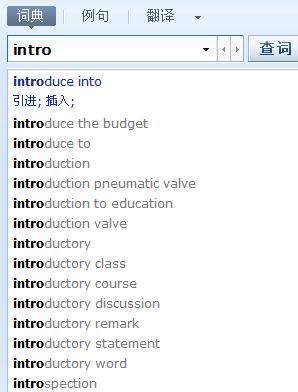
\includegraphics[scale=0.5]{img/ciba.eps}
        \caption{e-dictionary. All candidates starting with what user input are listed.}
        \label{fig:e-dict}
       \end{center}
\end{figure}

Typically such dictionary contains handres of thousands words, performs a whole
word search is expensive. Commercial software adopts complex approach, including
caching, indexing etc to speed up this process.

Similiar with e-dictionary, figure \ref{fig:word-completion} shows a popular
internet search engine, when user input someting, it will provide a candidate
lists, with all items start with what user has entered. And these candidates
are shown in an order of popularity. The more people search for a word, the
upper position it will be shown in the list.

\begin{figure}[htbp]
       \begin{center}
	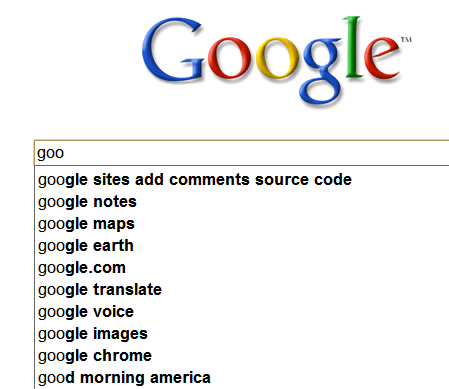
\includegraphics[scale=0.5]{img/adaptive-input.eps}
        \caption{Search engine. All candidates key words starting with what user input are listed.}
        \label{fig:word-completion}
       \end{center}
\end{figure}

In both case, we say the software provide a kind of word auto-completion support. 
In some mordern IDE, the editor can even helps user to auto-complete programmings. 

In this section, I'll show a very simple implementation of e-dictionary with Trie
and Patricia.
To simplify the problem, let us assume the dictionary only support English - English
information.

Typically, a dictionary contains a lot of key-value pairs, the keys are English
words or phrases, and the relative values are the meaning of the words.

We can store all words and their meanings to a Trie, the drawback for this 
approach is that it isn't space effective. We'll use Patricia as alternative
later on.

As an example, when user want to look up 'a', the dictionary does not only
return the meaning of then English word 'a', but also provide a list of 
candidate words, which are all start with 'a', including 'abandon', 'about',
'accent', 'adam', ... Of course all these words are stored in Trie.

If there are too many candidates, one solution is only display the top 10
words for the user, and if he like, he can browe more.

Below pseduo code resue the looking up program in previous sections and
Expand all potiential top N candidates.

\begin{algorithmic}
\STATE $TRIE-LOOK-UP-TOP-N(T, key, N)$
  \STATE $p \leftarrow TRIE-LOOK-UP'(T, key)$
  \RETURN $EXPAND-TOP-N(p, key, N)$
\end{algorithmic}

Note that we should modify the TRIE-LOOK-UP a bit, instead of return
the value of the node, TRIE-LOOK-UP' returns the node itself.

Another alternative is to use Patricia instead of Trie. It can save much
spaces.

\begin{algorithmic}
\STATE $PATRICIA-LOOK-UP-TOP-N(T, key, N)$
  \IF{$T = NIL$}
     \RETURN $NIL$ \ENDIF

  \STATE $prefix \leftarrow NIL$
  \REPEAT
    \STATE $match \leftarrow FALSE$
    \FOR{each $i$ in $CHILDREN(T)$}
      \IF{$key$ IS-PREFIX-OF $KEY(i)$}
        \RETURN $EXPAND-TOP-N(TREE(i), prefix, N)$
      \ENDIF
      \IF{$KEY(i)$ IS-PREFIX-OF $key$}
        \STATE $match \leftarrow TRUE$
        \STATE $key \leftarrow key$ subtract $KEY(i)$
        \STATE $T \leftarrow TREE(i)$
        \STATE $prefix \leftarrow prefix + KEY(i)$
        \STATE break
      \ENDIF
    \ENDFOR
  \UNTIL{$match = FALSE$}
  \RETURN $NIL$
\end{algorithmic}

\subsubsection*{An e-dictionary in Haskell}
In Haskell implementation, we provide a function named as findAll.
Thanks for the lazy evaluation support, findAll won't produce all candidates
words until we need them. we can use something like 'take 10 findAll'
to get the top 10 words easily.

findAll is given as the following.

\lstset{language=Haskell}
\begin{lstlisting}
findAll:: Trie a -> String -> [(String, a)]
findAll t [] = 
    case value t of
      Nothing -> enum (children t) 
      Just x  -> ("", x):(enum (children t))
    where
      enum [] = []
      enum (p:ps) = (mapAppend (fst p) (findAll (snd p) [])) ++ (enum ps)
findAll t (k:ks) = 
    case lookup k (children t) of
      Nothing -> []
      Just t' -> mapAppend k (findAll t' ks)

mapAppend x lst = map (\p->(x:(fst p), (snd p))) lst
\end{lstlisting}

function findAll take a Trie, a word to be looked up, it will output
a list of pairs, the first element of the pair is the candidate word,
the second element of the pair is the meaning of the word.

Compare with the find function of Trie, the none-trivial case is very similar.
We take a letter form the words to be looked up, if there is no child starting
with this letter, the program returns empty list. If there is such a child
starting with this letter, this child should be a candidate. We use function
mapAppend to add this letter in front of all elements of recusively founded
candidate words.

In case we consumed all letters, we next returns all potential words, which
means the program will traverse all children of the current node.

Note that only the node with value field not equal to 'None' is a meaningful
word in our dictionary. We need append the list with the right meaning.

With this function, we can constract a very simple dictionary and return
top 5 candidate to user. Here is the test program.

\begin{lstlisting}
testFindAll = "\nlook up a: " ++ (show $ take 5 $findAll t "a") ++
              "\nlook up ab: " ++ (show $ take 5 $findAll t "ab")
    where 
      t = fromList [
        ("a", "the first letter of English"), 
        ("an", "used instead of 'a' when the following word begins with" 
               "a vowel sound"), 
        ("another", "one more person or thing or an extra amount"), 
        ("abandon", "to leave a place, thing or person forever"),
        ("about", "on the subject of; connected with"),
        ("adam", "a character in the Bible who was the first man made by God"),
        ("boy", "a male child or, more generally, a male of any age"), 
        ("bodyl", "the whole physical structure that forms a person or animal"), 
        ("zoo", "an area in which animals, especially wild animals, are kept" 
                " so that people can go and look at them, or study them")]

main = do
    putStrLn testFindAll
\end{lstlisting}

This program will out put a result like this:
\begin{verbatim}
look up a: [("a","the first letter of English"),("an","used instead of 'a' 
when the following word begins with a vowel sound"),("another","one more 
person or thing or an extra amount"),("abandon","to leave a place, thing 
or person forever"),("about","on the subject of; connected with")]
look up ab: [("abandon","to leave a place, thing or person forever"),
("about","on the subject of; connected with")]
\end{verbatim}

The Trie solution wasts a lot of spaces. It is very easy to improve the above
program with Patricia. Below source code shows the Patricia approach.

\begin{lstlisting}
findAll' :: Patricia a -> Key -> [(Key, a)]
findAll' t [] =
    case value t of
      Nothing -> enum $ children t
      Just x  -> ("", x):(enum $ children t)
    where
      enum [] = []
      enum (p:ps) = (mapAppend' (fst p) (findAll' (snd p) [])) ++ (enum ps)
findAll' t k = find' (children t) k where
    find' [] _ = []
    find' (p:ps) k
          | (fst p) == k 
              = mapAppend' k (findAll' (snd p) [])
          | (fst p) `Data.List.isPrefixOf` k 
              = mapAppend' (fst p) (findAll' (snd p) (k `diff` (fst p)))
          | k `Data.List.isPrefixOf` (fst p) 
              = findAll' (snd p) []
          | otherwise = find' ps k
    diff x y = drop (length y) x

mapAppend' s lst = map (\p->(s++(fst p), snd p)) lst
\end{lstlisting}

If compare this program with the one implemented by Trie, we can find they are
very similiar to each other. In none-trivial case, we just examine each child
to see if any one match the key to be looked up. If one child is exactly equal
to the key, we then expand all its sub branches and put them to the candidate list.
If the child correspond to a prefix of the key, the program goes on find the 
the rest part of the key along this child and concatenate this prefix to all 
later results. If the current key is prefix to a child, the program will traverse
this child and return all its sub branches as candidate list.

This program can be tested with the very same case as above, and it will output
the same result.

\subsubsection*{An e-dictionary in Python}
In Haskell implementation, a function trie\_lookup\_N is provided to perform
search all top N candidate started with a given string.

\lstset{language=Python}
\begin{lstlisting}
def trie_lookup(t, key, n):
    if t is None:
        return None

    p = t
    for c in key:
        if not c in p.children:
            return None
        p=p.children[c]
    return expand(key, p, n)

def expand(prefix, t, n):
    res = []
    q = [(prefix, t)]
    while len(res)<n and len(q)>0:
        (s, p) = q.pop(0)
        if p.value is not None:
            res.append((s, p.value))
        for k, tr in p.children.items():
            q.append((s+k, tr))
    return res
\end{lstlisting}

Compare with the Trie lookup function, the first part of this program is almost
same. The difference part is after we successfully located the node which matches the key, all sub trees are expanded from this node in a bread-first search manner, and the top n candidates are returned. 

This program can be verified by below simple test cases.

\begin{lstlisting}
class LookupTest:
    def __init__(self):
        dict = {"a":"the first letter of English", \
           "an":"...same dict as in Haskell example"}
        self.tt = trie.map_to_trie(dict)

    def run(self):
        self.test_trie_lookup()

    def test_trie_lookup(self):
        print "test lookup top 5"
        print "search a ", trie_lookup(self.tt, "a", 5)
        print "search ab ", trie_lookup(self.tt, "ab", 5)
\end{lstlisting}

The test will output the following result.

\begin{verbatim}
test lookup to 5
search a  [('a', 'the first letter of English'), ('an', "used instead of 'a' 
when the following word begins with a vowel sound"), ('adam', 'a character in 
the Bible who was the first man made by God'), ('about', 'on the subject of; 
connected with'), ('abandon', 'to leave a place, thing or person forever')]
search ab  [('about', 'on the subject of; connected with'), ('abandon', 'to 
leave a place, thing or person forever')]
\end{verbatim}

To save the spaces, we can also implement such a dictionary search by using
Patricia.

\begin{lstlisting}
def patricia_lookup(t, key, n):
    if t is None:
        return None
    prefix = ""
    while(True):
        match = False
        for k, tr in t.children.items():
            if string.find(k, key) == 0: #is prefix of
                return expand(prefix+k, tr, n)
            if string.find(key, k) ==0:
                match = True
                key = key[len(k):]
                t = tr
                prefix += k
                break
        if not match:
            return None
\end{lstlisting}

In this program, we called Python string class to test if a string x is
prefix of a string y. In case we locate a node with the key we are looking
up is either equal of as prefix of the this sub tree, we expand it till
we find n candidates. Function expand() can be reused here.

We can test this program with the very same test cases and the results are
identical to the previous one.

\subsection{T9 input method}
Most mobile phones around year 2000 has a key pad. To edit a short message/email
with such key-pad, users typically have quite different experience from PC.
Because a mobile-phone key pad, or so called ITU-T key pad has few keys.
Figure {fig:itut-keypad} shows an example.

\begin{figure}[htbp]
       \begin{center}
	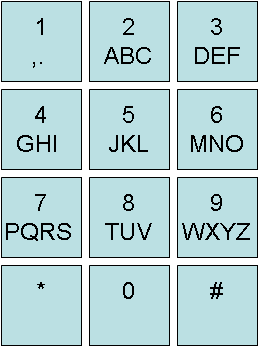
\includegraphics[scale=0.5]{img/itu-t.eps}
        \caption{an ITU-T keypad for mobile phone.}
        \label{fig:itut-keypad}
       \end{center}
\end{figure}

There are typical 2 methods to input an English word/phrase with ITU-T key pad.
For instance, if user wants to enter a word ``home'', He can press the key
in below sequence.

\begin{itemize}
\item Press key '4' twice to enter the letter 'h';
\item Press key '6' three times to enter the letter 'o';
\item Press key '6' twice to enter the letter 'm';
\item Press key '3' twice to enter the letter 'e';
\end{itemize}

Another high efficient way is to simplify the key press sequence like the
following.

\begin{itemize}
\item Press key '4', '6', '6', '3', word ``home'' appears on top of the candidate list;
\item Press key '*' to change a candidate word, so word ``good'' appears;
\item Press key '*' again to change another candidate word, next word ``gone'' apears;
\item ...
\end{itemize}

Compare these 2 method, we can see method 2 is much easier for the end user, and
it is operation efficient. The only overhead is to store a candidate words dictionary.

Method 2 is called as T9 input method, or predictive input method
\cite{wiki-t9}, \cite {wiki-predictive-text}. The abbreviation 'T9' stands
for 'textonym'. In this section, I'll show an example implementation of T9
by using Trie and Patricia.

In order to provide candidate words to user, a dictionary must be prepared
in advance. Trie or Patricia can be used to store the Dictionary. In the real
commercial software, complex indexing dictionary is used. We show the very 
simple Trie and Patricia only for illustration purpose.

Below pseduo code shows how to realize T9 with Trie.

\begin{algorithmic}
\STATE $TRIE-LOOK-UP-T9(T, key)$
  \STATE $PUSH-BACK(Q, NIL, key, T)$
  \STATE $r \leftarrow NIL$
  \WHILE{$Q$ is not empty}
    \STATE $p, k, t \leftarrow POP-FRONT(Q)$
    \STATE $i \leftarrow FIRST-LETTER(k)$
    \FOR{each $c$ in $T9-MAPPING(i)$}
      \IF{$c$ is in $CHILDREN(t)$}
        \STATE $k' \leftarrow k$ subtract $i$
        \IF{$k'$ is empty}
          \STATE $APPEND(r, p+c)$
        \ELSE
          \STATE $PUSH-BACK(Q, p+c, k', CHILDREN(t)[c])$
        \ENDIF
      \ENDIF
    \ENDFOR
  \ENDWHILE
  \RETURN $r$
\end{algorithmic}

This is actually a bread-first search program. It utilizes a queue to store
the current node and key string we are examing. The algorithm takes the first
digit from the key, looks up it in T9 mapping to get all English letters 
corresponding to this digit. For each letter, if it can be found in the children
of current node, the node along with the English string found so far are
push back to the queue. In case all digits are examined, a candidate is found.
We'll append this candidate to the result list. The loop will terminate when
the queue is empty.

Since Trie is not space effecitve, minor modification of the above program can
work with Patricia, which can help to save extra spaces.

\begin{algorithmic}
\STATE $PATRICIA-LOOK-UP-T9(T, key)$
  \STATE $PUSH-BACK(Q, NIL, key, T)$
  \STATE $r \leftarrow NIL$
  \WHILE{$Q$ is not empty}
    \STATE $p, k, t \leftarrow POP-FRONT(Q)$
    \FOR{each $child$ in $CHILDREN(t)$}
      \STATE $k' \leftarrow CONVERT-T9(KEY(child))$
      \IF{$k'$ IS-PREFIX-OF $k$}
        \IF{$k' = k$}
          \STATE $APPEND(r, p+KEY(child))$
        \ELSE
          \STATE $PUSH-BACK(Q, p+KEY(child), k-k', child)$
        \ENDIF
      \ENDIF
    \ENDFOR
  \ENDWHILE
  \RETURN $r$
\end{algorithmic}

\subsubsection*{T9 implemented in Haskell}

In Haskell, we first define a map from key pad to English letter. When user
input a key pad number sequence, we take each number and check from the Trie.
All children match the number should be investigated. Below is a Haskell 
program to realize T9 input.

\lstset{language=Haskell}
\begin{lstlisting}
mapT9 = [('2', "abc"), ('3', "def"), ('4', "ghi"), ('5', "jkl"), 
         ('6', "mno"), ('7', "pqrs"), ('8', "tuv"), ('9', "wxyz")]

lookupT9 :: Char -> [(Char, b)] -> [(Char, b)]
lookupT9 c children = case lookup c mapT9 of
        Nothing -> []
        Just s  -> foldl f [] s where
             f lst x = case lookup x children of
                 Nothing -> lst
                 Just t  -> (x, t):lst
        
-- T9-find in Trie
findT9:: Trie a -> String -> [(String, Maybe a)]
findT9 t [] = [("", Trie.value t)]
findT9 t (k:ks) = foldl f [] (lookupT9 k (children t))
    where
      f lst (c, tr) = (mapAppend c (findT9 tr ks)) ++ lst
\end{lstlisting}

findT9 is the main function, it takes 2 parameters, a Trie and a number
sequence string. In non-trivial case, it calls lookupT9 function to
examine all childrens which match the first number.

For each matched child, the program recursively calls findT9 on it with
the left numbers, and we use mapAppend to insert the currently finding letter
in front of all results. The program use foldl to combine all these together.

Function lookupT9 is used to filtered all possible children who match a
number. It first call lookup function on mapT9, so that a string of possible
English letters can be indentified. Next we call lookup for each candidate
letter to see if there is a child can match the letter. We use folderl to 
collect all such child together.

This proram can be verfied by using some simiple test cases.

\begin{lstlisting}
testFindT9 = "press 4: " ++ (show $ take 5 $ findT9 t "4")++
             "\npress 46: " ++ (show $ take 5 $ findT9 t "46")++
             "\npress 4663: " ++ (show $ take 5 $ findT9 t "4663")++
             "\npress 2: " ++ (show $ take 5 $ findT9 t "2")++
             "\npress 22: " ++ (show $ take 5 $ findT9 t "22")
    where
      t = Trie.fromList lst
      lst = [("home", 1), ("good", 2), ("gone", 3), ("hood", 4), 
             ("a", 5), ("another", 6), ("an", 7)]
\end{lstlisting}

The program will output below result.

\begin{verbatim}
press 4: [("g",Nothing),("h",Nothing)]
press 46: [("go",Nothing),("ho",Nothing)]
press 4663: [("gone",Just 3),("good",Just 2),("home",Just 1),("hood",Just 4)]
press 2: [("a",Just 5)]
press 22: []
\end{verbatim}

The value of each child is just for illustration, we can put empty value instead
and only returns candidate keys for a real input application.

Tries consumes to many spaces, we can provide a Patricia version as alternative.

\begin{lstlisting}
findPrefixT9' :: String -> [(String, b)] -> [(String, b)]
findPrefixT9' s lst = filter f lst where
    f (k, _) = (toT9 k) `Data.List.isPrefixOf` s

toT9 :: String -> String
toT9 [] = []
toT9 (x:xs) = (unmapT9 x mapT9):(toT9 xs) where
    unmapT9 x (p:ps) = if x `elem` (snd p) then (fst p) else unmapT9 x ps

findT9' :: Patricia a -> String -> [(String, Maybe a)]
findT9' t [] = [("", value t)]
findT9' t k = foldl f [] (findPrefixT9' k (children t)) 
    where
      f lst (s, tr) = (mapAppend' s (findT9' tr (k `diff` s))) ++ lst
      diff x y = drop (length y) x
\end{lstlisting}

In this program, we don't check one digit at a time, we take all the digit
sequence, and we examine all children of the Patricia node. For each dhild,
the program convert the prefix string to number sequence by using function 
toT9, if the result is prefix of what user input, we go on search in this 
child and append the prefix in front of all further results.

If we tries the same test case, we can find the result is a bit different.

\begin{verbatim}
press 4: []
press 46: [("go",Nothing),("ho",Nothing)]
press 466: []
press 4663: [("good",Just 2),("gone",Just 3),("home",Just 1),("hood",Just 4)]
press 2: [("a",Just 5)]
press 22: []
\end{verbatim}

If user press key '4', because the dictionary (represent by Patricia) doesn't
contain any candidates matches it, user will get an empty candidates list.
The same situation happens when he enters ``466''. In real input method 
implementation, such user epxerience isnt' good, because it displays nothing
although user presses the key serveral times. One improvement is to 
predict what user will input next by display a partial result. This can be 
easily achieved by modify the above program. (Hint: not only check
\begin{lstlisting}
findPrefixT9' s lst = filter f lst where
    f (k, _) = (toT9 k) `Data.List.isPrefixOf` s
\end{lstlisting}
but also check
\begin{lstlisting}
    f (k, _) = s `Data.List.isPrefixOf` (toT9 k)
\end{lstlisting}
)

\subsubsection*{T9 implementation in Python}

In Python implementation, T9 looking up is realized in a typical bread-first search algorithm as the following.

\lstset{language=Python}
\begin{lstlisting}
T9MAP={'2':"abc", '3':"def", '4':"ghi", '5':"jkl", \
       '6':"mno", '7':"pqrs", '8':"tuv", '9':"wxyz"}
                
def trie_lookup_t9(t, key):
    if t is None or key == "":
        return None
    q = [("", key, t)]
    res = []
    while len(q)>0:
        (prefix, k, t) = q.pop(0)
        i=k[0]
        if not i in T9MAP:
            return None #invalid input
        for c in T9MAP[i]:
            if c in t.children:
                if k[1:]=="":
                    res.append((prefix+c, t.children[c].value))
                else:
                    q.append((prefix+c, k[1:], t.children[c]))
    return res
\end{lstlisting}

Function trie\_lookup\_t9 check if the parameters are valide first. Then
it push the initial data into a queue. The program repeatly pop the item
from the queue, including what node it will examine next, the number sequence
string, and the alphabetic string it has been searched.

For each poped item, the program takes the next digit from the number
sequence, and looks up in T9 map to find the corresponding English letters.
With all these letters, if they can be found in the children of the current
node, we'll push this child along with the updated number sequence string
and updated alphabetic string into the queue. In case we process all 
numbers, we find a candidate result.

We can verify the above program with the following test cases.

\begin{lstlisting}
class LookupTest:
    def __init__(self):
        t9dict = ["home", "good", "gone", "hood", "a", "another", "an"]
        self.t9t = trie.list_to_trie(t9dict)

    def test_trie_t9(self):
        print "search 4 ", trie_lookup_t9(self.t9t, "4")
        print "search 46 ", trie_lookup_t9(self.t9t, "46")
        print "search 4663 ", trie_lookup_t9(self.t9t, "4663")
        print "search 2 ", trie_lookup_t9(self.t9t, "2")
        print "search 22 ", trie_lookup_t9(self.t9t, "22")
\end{lstlisting}

If we run the test, it will output a very same result as the above Haskell
program.

\begin{verbatim}
search 4  [('g', None), ('h', None)]
search 46  [('go', None), ('ho', None)]
search 4663  [('gone', None), ('good', None), ('home', None), ('hood', None)]
search 2  [('a', None)]
search 22  []
\end{verbatim}

To save the spaces, Patricia can be used instead of Trie.

\begin{lstlisting}
def patricia_lookup_t9(t, key):
    if t is None or key == "":
        return None
    q = [("", key, t)]
    res = []
    while len(q)>0:
        (prefix, key, t) = q.pop(0)
        for k, tr in t.children.items():
            digits = toT9(k)
            if string.find(key, digits)==0: #is prefix of
                if key == digits:
                    res.append((prefix+k, tr.value))
                else:
                    q.append((prefix+k, key[len(k):], tr))
    return res
\end{lstlisting}

Compare to the implementation with Trie, they are very similiar. We also 
used a bread-first search approach. The different part is that we convert
the string of each child to number sequence string according to T9 mapping.
if it is prefix of the key we are looking for, we push this child along with
updated key and prefix. In case we examined all digits, we find a candidate
result.

The convert function is a reverse mapping process as below.
\begin{lstlisting}
def toT9(s):
    res=""
    for c in s:
        for k, v in T9MAP.items():
            if string.find(v, c)>=0:
                res+=k
                break
        #error handling skipped.
    return res
\end{lstlisting}

For illustration purpose, the error handling for invalid letters is skipped.
If we feed the program with the same test cases, we can get a result as the 
following.

\begin{verbatim}
search 4  []
search 46  [('go', None), ('ho', None)]
search 466  []
search 4663  [('good', None), ('gone', None), ('home', None), ('hood', None)]
search 2  [('a', None)]
search 22  []
\end{verbatim}

The result is slightly different from the one output by Trie. The reason is
as same as what we analyzed in Haskell implementation. It is easily to modify
the program to output a similar result.

% ================================================================
%                 Appendix
% ================================================================
\section{Appendix} \label{appendix}
%\appendix
All programs provided along with this article. They are free for downloading.
\begin{itemize}
\item IntTrie.hs, Haskell version of little-endian integer Trie, with test cases. I compiled
and tested it with GHC 6.10.4.
\item inttrie.cpp,
\item inttrie.py, Python version of little-endian integer Trie, with test cases. Tested
with Python 2.5.1
\item inttrie.scm,
\item IntPatricia.hs, integer Patricia tree implemented in
Haskell. Tested with GCH 6.10.4. 
\item intpatricia.cpp,
\item intpatricia.py, integer Patricia tree implemented in
Python. Tested with Python 2.5.1
\item intpatricia.scm
\item trie.c, Alphabetic Trie only for lowercase English language,
implemented in ANSI C. Tested with GNU GCC 3.4.4
\item Trie.hs, Alphabetic Trie, implemented in Haskell. Tested with
GHC 6.10.4.
\item trie.cpp,
\item trie.py, Alphabetic Trie, implemented in Python. Tested with
Python 2.5.1.
\item trie.scm,
\item Patricia.hs,
\item patricia.cpp,
\item patricia.py,
\item patricia.scm,
\item xxx.scm, Scheme version of xxxx and test cases. Tested
with MIT/Scheme 14.9
\end{itemize}

Besides them, I use graphviz to draw most of the figures in this post. In order to
translate the Trie, Patrica and Suffix Tree output to dot language scripts. I wrote a python program.
it can be used like this.

\begin{verbatim}
trie2dot.py -o foo.dot -t patricia "1:x, 4:y, 5:z"
trie2dot.py -o foo.dot -t trie "001:one, 101:five, 100:four"
\end{verbatim}

This helper scripts can also be downloaded with this article.

download position: http://sites.google.com/site/algoxy/trie/trie.zip

\begin{thebibliography}{99}

\bibitem{CLRS}
Thomas H. Cormen, Charles E. Leiserson, Ronald L. Rivest and Clifford Stein. 
``Introduction to Algorithms, Second Edition''. ISBN:0262032937. The MIT Press. 2001

\bibitem{okasaki-int-map}
Chris Okasaki and Andrew Gill. ``Fast Mergeable Integer
Maps''. Workshop on ML, September 1998, pages 77-86, http://www.cse.ogi.edu/~andy/pub/finite.htm

\bibitem{patricia-morrison}
D.R. Morrison, ``PATRICIA -- Practical Algorithm To Retrieve  Information Coded In Alphanumeric", Journal of the ACM, 15(4), October 1968, pages 514-534.

\bibitem{wiki-suffix-tree}
Suffix Tree, Wikipedia. http://en.wikipedia.org/wiki/Suffix\_tree

\bibitem{wiki-trie}
Trie, Wikipedia. http://en.wikipedia.org/wiki/Trie

\bibitem{wiki-t9}
T9 (predictive text), Wikipedia. http://en.wikipedia.org/wiki/T9\_(predictive\_text)

\bibitem{wiki-predictive-text}
Predictive text, Wikipedia. http://en.wikipedia.org/wiki/Predictive\_text

\end{thebibliography}

\ifx\wholebook\relax\else
\end{document}
\fi
